% Options for packages loaded elsewhere
\PassOptionsToPackage{unicode}{hyperref}
\PassOptionsToPackage{hyphens}{url}
\PassOptionsToPackage{dvipsnames,svgnames,x11names}{xcolor}
%
\documentclass[
]{agujournal2019}

\usepackage{amsmath,amssymb}
\usepackage{iftex}
\ifPDFTeX
  \usepackage[T1]{fontenc}
  \usepackage[utf8]{inputenc}
  \usepackage{textcomp} % provide euro and other symbols
\else % if luatex or xetex
  \usepackage{unicode-math}
  \defaultfontfeatures{Scale=MatchLowercase}
  \defaultfontfeatures[\rmfamily]{Ligatures=TeX,Scale=1}
\fi
\usepackage{lmodern}
\ifPDFTeX\else  
    % xetex/luatex font selection
\fi
% Use upquote if available, for straight quotes in verbatim environments
\IfFileExists{upquote.sty}{\usepackage{upquote}}{}
\IfFileExists{microtype.sty}{% use microtype if available
  \usepackage[]{microtype}
  \UseMicrotypeSet[protrusion]{basicmath} % disable protrusion for tt fonts
}{}
\makeatletter
\@ifundefined{KOMAClassName}{% if non-KOMA class
  \IfFileExists{parskip.sty}{%
    \usepackage{parskip}
  }{% else
    \setlength{\parindent}{0pt}
    \setlength{\parskip}{6pt plus 2pt minus 1pt}}
}{% if KOMA class
  \KOMAoptions{parskip=half}}
\makeatother
\usepackage{xcolor}
\setlength{\emergencystretch}{3em} % prevent overfull lines
\setcounter{secnumdepth}{5}
% Make \paragraph and \subparagraph free-standing
\makeatletter
\ifx\paragraph\undefined\else
  \let\oldparagraph\paragraph
  \renewcommand{\paragraph}{
    \@ifstar
      \xxxParagraphStar
      \xxxParagraphNoStar
  }
  \newcommand{\xxxParagraphStar}[1]{\oldparagraph*{#1}\mbox{}}
  \newcommand{\xxxParagraphNoStar}[1]{\oldparagraph{#1}\mbox{}}
\fi
\ifx\subparagraph\undefined\else
  \let\oldsubparagraph\subparagraph
  \renewcommand{\subparagraph}{
    \@ifstar
      \xxxSubParagraphStar
      \xxxSubParagraphNoStar
  }
  \newcommand{\xxxSubParagraphStar}[1]{\oldsubparagraph*{#1}\mbox{}}
  \newcommand{\xxxSubParagraphNoStar}[1]{\oldsubparagraph{#1}\mbox{}}
\fi
\makeatother


\providecommand{\tightlist}{%
  \setlength{\itemsep}{0pt}\setlength{\parskip}{0pt}}\usepackage{longtable,booktabs,array}
\usepackage{calc} % for calculating minipage widths
% Correct order of tables after \paragraph or \subparagraph
\usepackage{etoolbox}
\makeatletter
\patchcmd\longtable{\par}{\if@noskipsec\mbox{}\fi\par}{}{}
\makeatother
% Allow footnotes in longtable head/foot
\IfFileExists{footnotehyper.sty}{\usepackage{footnotehyper}}{\usepackage{footnote}}
\makesavenoteenv{longtable}
\usepackage{graphicx}
\makeatletter
\def\maxwidth{\ifdim\Gin@nat@width>\linewidth\linewidth\else\Gin@nat@width\fi}
\def\maxheight{\ifdim\Gin@nat@height>\textheight\textheight\else\Gin@nat@height\fi}
\makeatother
% Scale images if necessary, so that they will not overflow the page
% margins by default, and it is still possible to overwrite the defaults
% using explicit options in \includegraphics[width, height, ...]{}
\setkeys{Gin}{width=\maxwidth,height=\maxheight,keepaspectratio}
% Set default figure placement to htbp
\makeatletter
\def\fps@figure{htbp}
\makeatother
% definitions for citeproc citations
\NewDocumentCommand\citeproctext{}{}
\NewDocumentCommand\citeproc{mm}{%
  \begingroup\def\citeproctext{#2}\cite{#1}\endgroup}
\makeatletter
 % allow citations to break across lines
 \let\@cite@ofmt\@firstofone
 % avoid brackets around text for \cite:
 \def\@biblabel#1{}
 \def\@cite#1#2{{#1\if@tempswa , #2\fi}}
\makeatother
\newlength{\cslhangindent}
\setlength{\cslhangindent}{1.5em}
\newlength{\csllabelwidth}
\setlength{\csllabelwidth}{3em}
\newenvironment{CSLReferences}[2] % #1 hanging-indent, #2 entry-spacing
 {\begin{list}{}{%
  \setlength{\itemindent}{0pt}
  \setlength{\leftmargin}{0pt}
  \setlength{\parsep}{0pt}
  % turn on hanging indent if param 1 is 1
  \ifodd #1
   \setlength{\leftmargin}{\cslhangindent}
   \setlength{\itemindent}{-1\cslhangindent}
  \fi
  % set entry spacing
  \setlength{\itemsep}{#2\baselineskip}}}
 {\end{list}}
\usepackage{calc}
\newcommand{\CSLBlock}[1]{\hfill\break\parbox[t]{\linewidth}{\strut\ignorespaces#1\strut}}
\newcommand{\CSLLeftMargin}[1]{\parbox[t]{\csllabelwidth}{\strut#1\strut}}
\newcommand{\CSLRightInline}[1]{\parbox[t]{\linewidth - \csllabelwidth}{\strut#1\strut}}
\newcommand{\CSLIndent}[1]{\hspace{\cslhangindent}#1}

\usepackage{url} %this package should fix any errors with URLs in refs.
\usepackage{lineno}
\usepackage[inline]{trackchanges} %for better track changes. finalnew option will compile document with changes incorporated.
\usepackage{soul}
\linenumbers
\makeatletter
\@ifpackageloaded{caption}{}{\usepackage{caption}}
\AtBeginDocument{%
\ifdefined\contentsname
  \renewcommand*\contentsname{Table of contents}
\else
  \newcommand\contentsname{Table of contents}
\fi
\ifdefined\listfigurename
  \renewcommand*\listfigurename{List of Figures}
\else
  \newcommand\listfigurename{List of Figures}
\fi
\ifdefined\listtablename
  \renewcommand*\listtablename{List of Tables}
\else
  \newcommand\listtablename{List of Tables}
\fi
\ifdefined\figurename
  \renewcommand*\figurename{Figure}
\else
  \newcommand\figurename{Figure}
\fi
\ifdefined\tablename
  \renewcommand*\tablename{Table}
\else
  \newcommand\tablename{Table}
\fi
}
\@ifpackageloaded{float}{}{\usepackage{float}}
\floatstyle{ruled}
\@ifundefined{c@chapter}{\newfloat{codelisting}{h}{lop}}{\newfloat{codelisting}{h}{lop}[chapter]}
\floatname{codelisting}{Listing}
\newcommand*\listoflistings{\listof{codelisting}{List of Listings}}
\makeatother
\makeatletter
\makeatother
\makeatletter
\@ifpackageloaded{caption}{}{\usepackage{caption}}
\@ifpackageloaded{subcaption}{}{\usepackage{subcaption}}
\makeatother

\ifLuaTeX
  \usepackage{selnolig}  % disable illegal ligatures
\fi
\usepackage{bookmark}

\IfFileExists{xurl.sty}{\usepackage{xurl}}{} % add URL line breaks if available
\urlstyle{same} % disable monospaced font for URLs
\hypersetup{
  pdftitle={Cumulative and individual impacts of the human footprint on similarity to high ecological integrity reference states.},
  pdfauthor={Evan Muise; Nicholas Coops; Txomin Hermosilla; Chris Mulverhill; Cole Burton; Stephen Ban},
  pdfkeywords={Protected areas, Coarsened exact matching, Reference
states, Remote sensing, Ecosystem structure, Ecosystem
function, Anthropogenic pressure, Human footprint},
  colorlinks=true,
  linkcolor={blue},
  filecolor={Maroon},
  citecolor={Blue},
  urlcolor={Blue},
  pdfcreator={LaTeX via pandoc}}



\draftfalse

\begin{document}
\title{Cumulative and individual impacts of the human footprint on
similarity to high ecological integrity reference states.}

\authors{Evan Muise\affil{1}, Nicholas Coops\affil{1}, Txomin
Hermosilla\affil{2}, Chris Mulverhill\affil{1}, Cole
Burton\affil{1}, Stephen Ban\affil{3}}
\affiliation{1}{Department of Forest Resource Management, University of
British Columbia, Vancouver, British Columbia,
Canada, }\affiliation{2}{Canadian Forest Service (Pacific Forestry
Centre), Natural Resources Canada, Victoria, British Columbia,
Canada, }\affiliation{3}{BC Parks, Government of British Columbia,
Victoria, British Columbia, Canada, }
\correspondingauthor{Evan Muise}{evanmuis@student.ubc.ca}


\begin{abstract}
Forests with high ecological integrity have natural or near natural
ecosystem structure, function, and composition, are home to large
amounts of biodiversity, and provide integral ecosystem services.
Anthropogenic pressures such as habitat loss, overexploitation, and land
use changes are leading to the degradation or loss of high integrity
forests. As a result, it is important to be able to locate and assess
the quality of forests stands across wide swaths of land. Remote sensing
is inreasingly capable of making these assessments, through new data
such as wall to wall metrics of forest structure and productivity. In
this paper, we demonstrate a method to assess similarity to known high
quality reference states using coarsened exact matching and the sigma
dissimilarity metric. Using this dissimilarity metric, we can assess how
far, in structural and functional space, every forest stand across
Vancouver Island is to a comparable forest found in the oldest and
largest protected area on the island, Strathcona Provincial Park. We
further assess how cumulative and individual anthropogenic pressures are
influencing ecological dissimilarity. We found that cumulative
anthropogenic pressures influence the vertical layering of forests
(canopy height and structural complexity), but do not influence forest
energy availability or energy seasonality. Further, individual
anthropogenic pressures increase dissimilarity for the majority of
forest structural attributes, and population density reduces similarity
to highly seasonal forests. Our results demonstrate that applying strict
matching procedures and the sigma dissimilarity metric can be used to
assess ecosystem similarity, which could be useful when examining
locations of rare ecosystems under large amounts of anthropogenic
pressure. Further, we demonstrate that vertical forest structural
attributes which area strongly related to biodiversity via niche
availability and resource partitioning are influenced negatively by
anthropogenic pressures.
\end{abstract}





\section{Introduction}\label{introduction}

A global biodiversity crisis is currently underway, driven by
anthropogenic changes to natural habitats (Dirzo and Raven, 2003).
Pressures such as climate change, overexploitation, and invasive species
are leading to species extinctions (Thomas et al., 2004; Urban, 2015)
and the homogenization of biological communities (McGill et al., 2015).
The Kunming-Montreal Global Biodiversity Framework (GBF) was adopted in
December 2022 with the goal of restoring and safeguarding global
biodiversity (Convention on Biological Diversity, 2023). Targets within
this framework include restoring 30\% of all degraded ecosystems,
protecting 30\% of the Earth's terrestrial, inland water, and marine
areas, and achieving no loss of high biodiversity importance areas,
including high ecological integrity ecosystems (Convention on Biological
Diversity, 2023). In the terrestrial environment, forest biomes have
been shown to harbour the largest amount of biodiversity (Cardinale et
al., 2012; Myers, 1988; Pimm and Raven, 2000), and provide key ecosystem
services (Thompson et al., 2009). To provide these services, it is
integral that these forest ecosystems are in good ecological condition,
as represented by natural or near-natural levels of forest structure,
function, and composition, often referred to as having high ecological
integrity (Marín et al., 2021).

While understanding forest condition is a key aspect of understanding
biodiversity and the provision of ecosystem services due to their
inherent linkages (Cardinale et al., 2012; Hansen et al., 2021; Marín et
al., 2021), it is challenging to obtain suitable field-derived data
across extensive land areas due to the significant financial and
temporal costs associated with large-scale field campaigns. Remote
sensing data, however, can provide a efficient and cost-effective
alternative to field data, offering access to new spatially explicit and
comprehensive datasets that can be linked to ecological condition, with
additional metrics being proposed at a rapid pace (Pereira et al., 2013;
Radeloff et al., 2024; Skidmore et al., 2021). Advances in lidar
technologies and modelling methods are enabling the generation of
wall-to-wall estimates of forest stand structure for across entire
countries (Becker et al., 2023; Matasci et al., 2018a; Matasci et al.,
2018b), which serve as a more detailed indicator of ecosystem structure
than the often previously used landscape fragmentation metrics (Andrew
et al., 2012). Productivity metrics have been employed as a proxy for
ecosystem function for many years (Pettorelli et al., 2018, 2005), with
new Landsat-derived datasets providing integrative annual estimates of
energy availability at a 30 m spatial resolution (Radeloff et al., 2024;
Radeloff et al., 2019; Razenkova et al., n.d.). Remote sensing is
quickly providing access to a vast array of datasets suitable for
monitoring the various facets of biodiversity and ecological condition
(Noss, 1990; Pereira et al., 2013; Skidmore et al., 2021). The
integration of these datasets with information pertaining to the
location of known high-ecological-integrity forests enables researchers
and managers to identify high-quality forest reference states across
entire jurisdictions, even in the presence of anthropogenic pressures.

Ecological reference states represent baseline conditions of ecosystems,
serving as a benchmark for assessing ecological health and guiding
restoration efforts (Nielsen et al., 2007). The application of
counterfactual thinking, which entails considering the potenital state
of an ecosystem in the absence of anthropogenic pressures (Ferraro,
2009) can be instrumental for mapping high-integrity forests. Approaches
such as coarsened exact matching (Iacus et al., 2012), can be used to
facilitate comparisons between forest stands and their hypothetical
reference states. These methods account for confounding environmental
variables, thereby ensuring that all forests are compared to an
appropriate reference state. Identifying a suitable reference state can
be difficult, however there are methods which can be used to approximate
high-integrity reference conditions. Historical reference states can be
used when an ecosystem has a large depth of temporal data to compare to,
however, it is not always guaranteed that an ecosystem can be restored
to these historical norms due to changing climates (Balaguer et al.,
2014; McNellie et al., 2020). Other proposed methods for delineating
baseline conditions include protected areas (Arcese and Sinclair, 1997),
and empirical estimates of the reference state generated by modelling
outcomes (oftentimes species abundances and occurrence) in the absence
of anthropogenic disturbance (Nielsen et al., 2007).

Protected areas, specifically designed for biodiversity conservation,
are frequently faced with lower levels anthropogenic pressure as a
result of biases in their placement (Joppa and Pfaff, 2009; Muise et
al., 2022). In forested ecosystems, over time this leads to undisturbed
high-integrity forests remaining within protected areas due to their
natural disturbance regimes and a lack of anthropogenic pressures
(Brumelis et al., 2011). These high-integrity forests, situated within
protected areas, can serve as effective ecological baselines (Arcese and
Sinclair, 1997). When suitably matched to unprotected areas, they can be
used as a reference state to assess the differences between all forests
and their high-integrity counterparts (Ferraro, 2009). Further,
protected areas and undisturbed ecosystems such as intact forest
landscapes have been shown to have increased structural densities when
compared to other ecosystems (Li et al., 2023; Muise et al., 2022).

Anthropogenic pressure such as increased road densities (Nielsen et al.,
2007), harvesting and fossil fuel exploration activities leading to edge
effects (Bourgoin et al., 2024; Harfoot et al., 2018), and other
human-induced disturbances (Liira et al., 2007) have been shown to
influence forest structure. Novel datasets such as the Forest Structural
Condition Index have been developed which integrate both structure and
anthropogenic pressure into an index which identifies ecosystems of high
conservation value, with high structural complexity and low
anthropogenic pressure (Hansen et al., 2019). The impacts of
anthropocentric pressure on forest functioning and energy availability
is less frequently assessed. Hedwall et al. (2019) assessed plant
community shifts under anthropogenic pressures in the boreal forests of
Sweden, and hypothesized that changed communities may affect forest
functioning. Grantham et al. (2020) used forest extent and arrangement,
alongside pressure datasets, to assess ecosystem integrity, with
expectations that high-integrity ecosystems will retain high levels of
ecosystem functioning. However, to our knowledge, direct impacts of
anthropogenic pressures on forest ecosystem function have not been
assessed at a landscape scale.

We proposed a novel, data-driven, approach to identify high-integrity
forests based on various satellite-derived metrics of ecosystem
condition, and calculate the degree of structural and functional
similarity for unprotected areas to high-integrity forests found on
Vancouver Island, British Columbia, Canada. We use a strict matching
approach to ensure ecological similarity, and choose the highest 10\% of
metric values across variables that are known to be correlated with
ecological condition and biodiversity. We then calculate ecological
similarity using sigma dissimilarity (Mahony et al., 2017) alongside
human footprint layers developed by Hirsh-Pearson et al. (2022) to
assess the influence of anthropogenic pressure of ecological integrity
by cumulative and individual pressures. Further, we compare the
similarity metrics between ecological structure and function to identify
linkages between ecological similartiy of forest structure and forest
functioning, while accounting for the presence of anthropogenic
pressures.

\section{Methods}\label{methods}

\subsection{Study Area}\label{study-area}

We focus on the forested areas of Vancouver Island, British Columbia,
Canada. Vancouver island has approximately 31285 km\textsuperscript{2}
of land area, of which 79.5\% is forested. The dominant forest species
on Vancouver Island are Douglas-fir (\emph{Pseudotsuga menziesii}),
western red cedar (\emph{Thuja plicata}), western hemlock (\emph{Tsuga
heterophylla}), yellow cedar (\emph{Chamaecyparis nootkatensis}), and
Sitka spruce (\emph{Picea sitchensis}) (Burns, 1990). British Columbia
generally has at temperate maritime climate, with mild, wet winters, and
cool, dry summers. There are four ecosystems on Vancouver Island as
defined by British Columbia's biogeoclimatic ecosystem classification
(BEC) framework (Pojar et al., 1987), Coastal Western Hemlock (CWH),
Mountain Hemlock (MH), Coastal Douglas Fir (CDF), and Coastal
Mountain-heather Alpine (CMA), which are broadly delineated based on
soil, climate, and elevation. Forestry is an important industry on
Vancouver Island, while fires are historically rare and low severity
(Daniels and Gray, 2006).

\phantomsection\label{cell-fig-study}
\begin{figure}[H]

\centering{

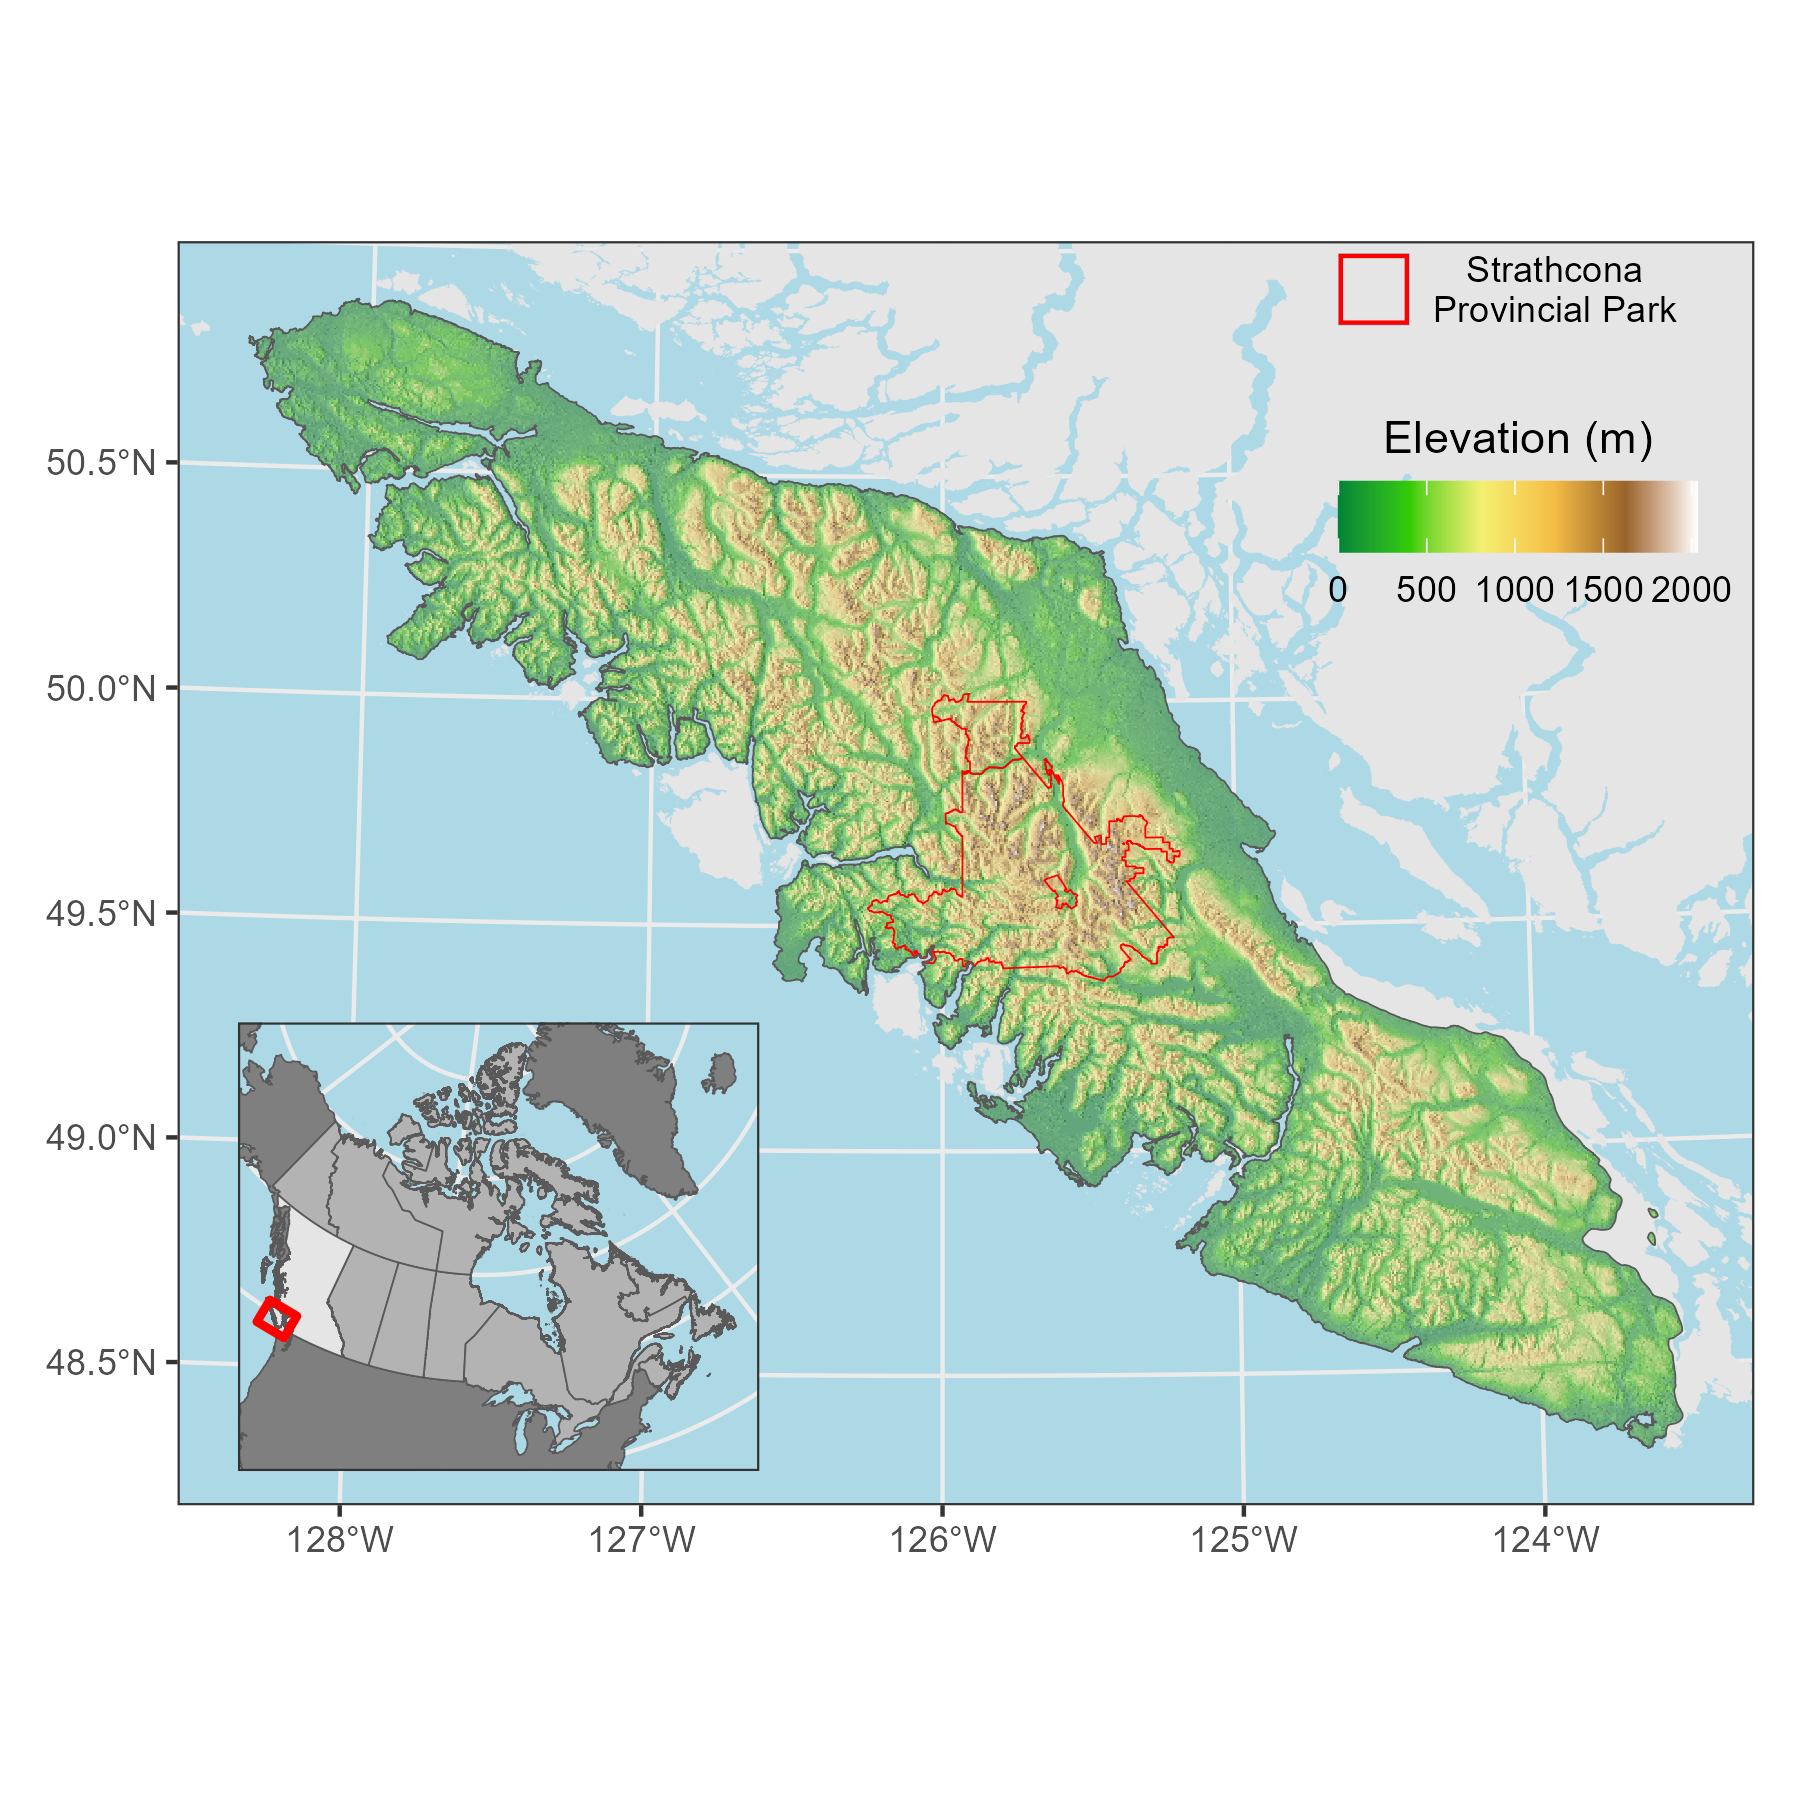
\includegraphics[width=6in,height=\textheight]{strathcona/figures/study_area.png}

}

\caption{\label{fig-study}Study area on Vancouver Island, British
Columbia, Canada, including the location of Strathcona Provincial Park.}

\end{figure}%

\subsection{Data}\label{data}

\subsubsection{Reference State}\label{reference-state}

We defined our reference state as the forested area of Strathcona Park.
We chose Strathcona Park as a temporal and protected area reference
state, as the oldest and largest (2480 km\textsuperscript{2}) protected
area in British Columbia. Strathcona Park was established in 1911, and
80\% of the park is preserved as wilderness area and designated as
Nature Conservancy Areas under the \emph{Park Act} ({``Park {Act},''}
n.d.). The park contains three BEC zones, CWH, MH, and CMA, but does not
include CDF, which is only found in the southern portion of the island.
Due to this, we do not include CDF in our analysis.

\subsubsection{Forest Structure}\label{forest-structure}

Wall-to-wall, 30 m forest structure metrics (canopy height, canopy
cover, structural complexity, and aboveground biomass) were generated by
Matasci et al. (2018a) for 2015 across the forested landscape of British
Columbia. This data was generated by using a random forest-kNN approach,
imputing airborne laser scanning derived forest structural attributes
across the entirety of Canada using Landsat-derived best-available-pixel
(BAP) composites (Hermosilla et al., 2016; White et al., 2014) and
topographic information (Matasci et al., 2018a; Matasci et al., 2018b).
The BAP composites were derived by selecting optical observations from
the Landsat archive (including Landsat-5 Thematic Mapper, Landsat-7
Enhanced Thematic Mapper Plus, and Landsat-8 Operational Land Imager
imagery) over the course of the growing season, considering atmospheric
effects (haze, clouds, cloud shadows) and distance from the desired
composite date (in this case, August 31st). Details on the pixel scoring
method can be found in White et al. (2014). The BAP composites were
further refined by using a spectral trend analysis on the normalized
burn ratio to remove noise, and missing pixels are infilled using
temporally-interpolated values. This procedure results in gap-free,
surface-reflectance image composites (Hermosilla et al., 2015), which
are used as the primary dataset to impute forest structural attributes
(Matasci et al., 2018a; Matasci et al., 2018b).

\subsubsection{Forest Function}\label{forest-function}

For our forest ecosystem function dataset, we calculated the Dynamic
Habitat Indices (Radeloff et al., 2019) using Landsat data on Google
Earth Engine (Gorelick et al., 2017), following the methodology of
Razenkova et al. (n.d.). Briefly, we created a synthetic year of NDVI
composites using all available Landsat imagery from 2011-2020 (centred
on 2015). We used the Landsat QA band derived from the fmask algorithm
(Zhu and Woodcock, 2012) to filter out erroneous pixels, such as clouds
and cloud shadows. Monthly NDVI values were calculated by taking the
median of each month's NDVI observations, ignoring the year the image
was acquired. This allows us to generate the DHIs at spatial resolution
of 30 m, while accounting for the lower temporal resolution of the
Landsat series when compared to the more commonly used MODIS satellites
(Razenkova et al., n.d.). The DHIs are calculated as the sum (Cumulative
DHI), minimum (Minimum DHI), and coefficient of variation (Variation
DHI) of these monthly observations. The three DHIs have been shown to be
indicative of biodiversity overa range of scales (Radeloff et al., 2019;
Razenkova et al., 2022) and extents (Coops et al., 2019, 2009) for a
variety of clades (Michaud et al., 2014; Suttidate et al., 2021). In
this study, we focus on the Cumulative and Variation DHIs, as the
minimum DHI is consistently 0 due to the presence of snow.

\subsubsection{Anthropogenic Pressures}\label{anthropogenic-pressures}

We use the Canadian Human Footprint as developed by Hirsh-Pearson et al.
(2022). The Canadian Human Footprint is an additive pressure map
generated by summing the 12 different anthropogenic pressures (built
environments, crop land, pasture land, population density, nighttime
lights, railways, roads, navigable waterways, dams and associated
reservoirs, mining activity, oil and gas, and forestry), which ranges
from zero to 55 for any cell across Canada. This cumulative dataset is
also distributed with Canada-wide individual pressure values
(Hirsh-Pearson et al., n.d.). Here, we focus on the overall cumulative
pressure map and four individual pressures: population density, built
environments, roads, and forestry. We selected these pressures as some
others (oil and gas; railroads) are not present on Vancouver Island, and
others, such as pasture land and crop land do not coincide with forested
areas.

\subsubsection{Covariates}\label{covariates}

In our matching procedure (see Section~\ref{sec-sim}) we use two core
datasets as our matching covariates. Firstly, we use a 30 m digital
elevation model and derived slope dataset from the Advanced Spaceborne
Thermal Emission and Reflection Radiometer (ASTER) Version 2 GDEM
product (Tachikawa et al., 2011). We also match on four climate
variables; mean annual precipitation (MAP), mean annual temperature
(MAT), mean warmest month temperature (MWMT), and mean coldest month
temperature (MCMT) calculated from 1990-2020 climate normals using the
ClimateNA software package at a 1 km spatial resolution, and downsampled
to 30 m using cubic spline resampling in the \textbf{terra} (version
1.7-71) R package (Hijmans, 2024) in R (R Core Team, 2024 version
4.4.1). A visualization of one of each input dataset can be found in
Figure Figure~\ref{fig-data}.

\phantomsection\label{cell-fig-data}
\begin{figure}[H]

\centering{

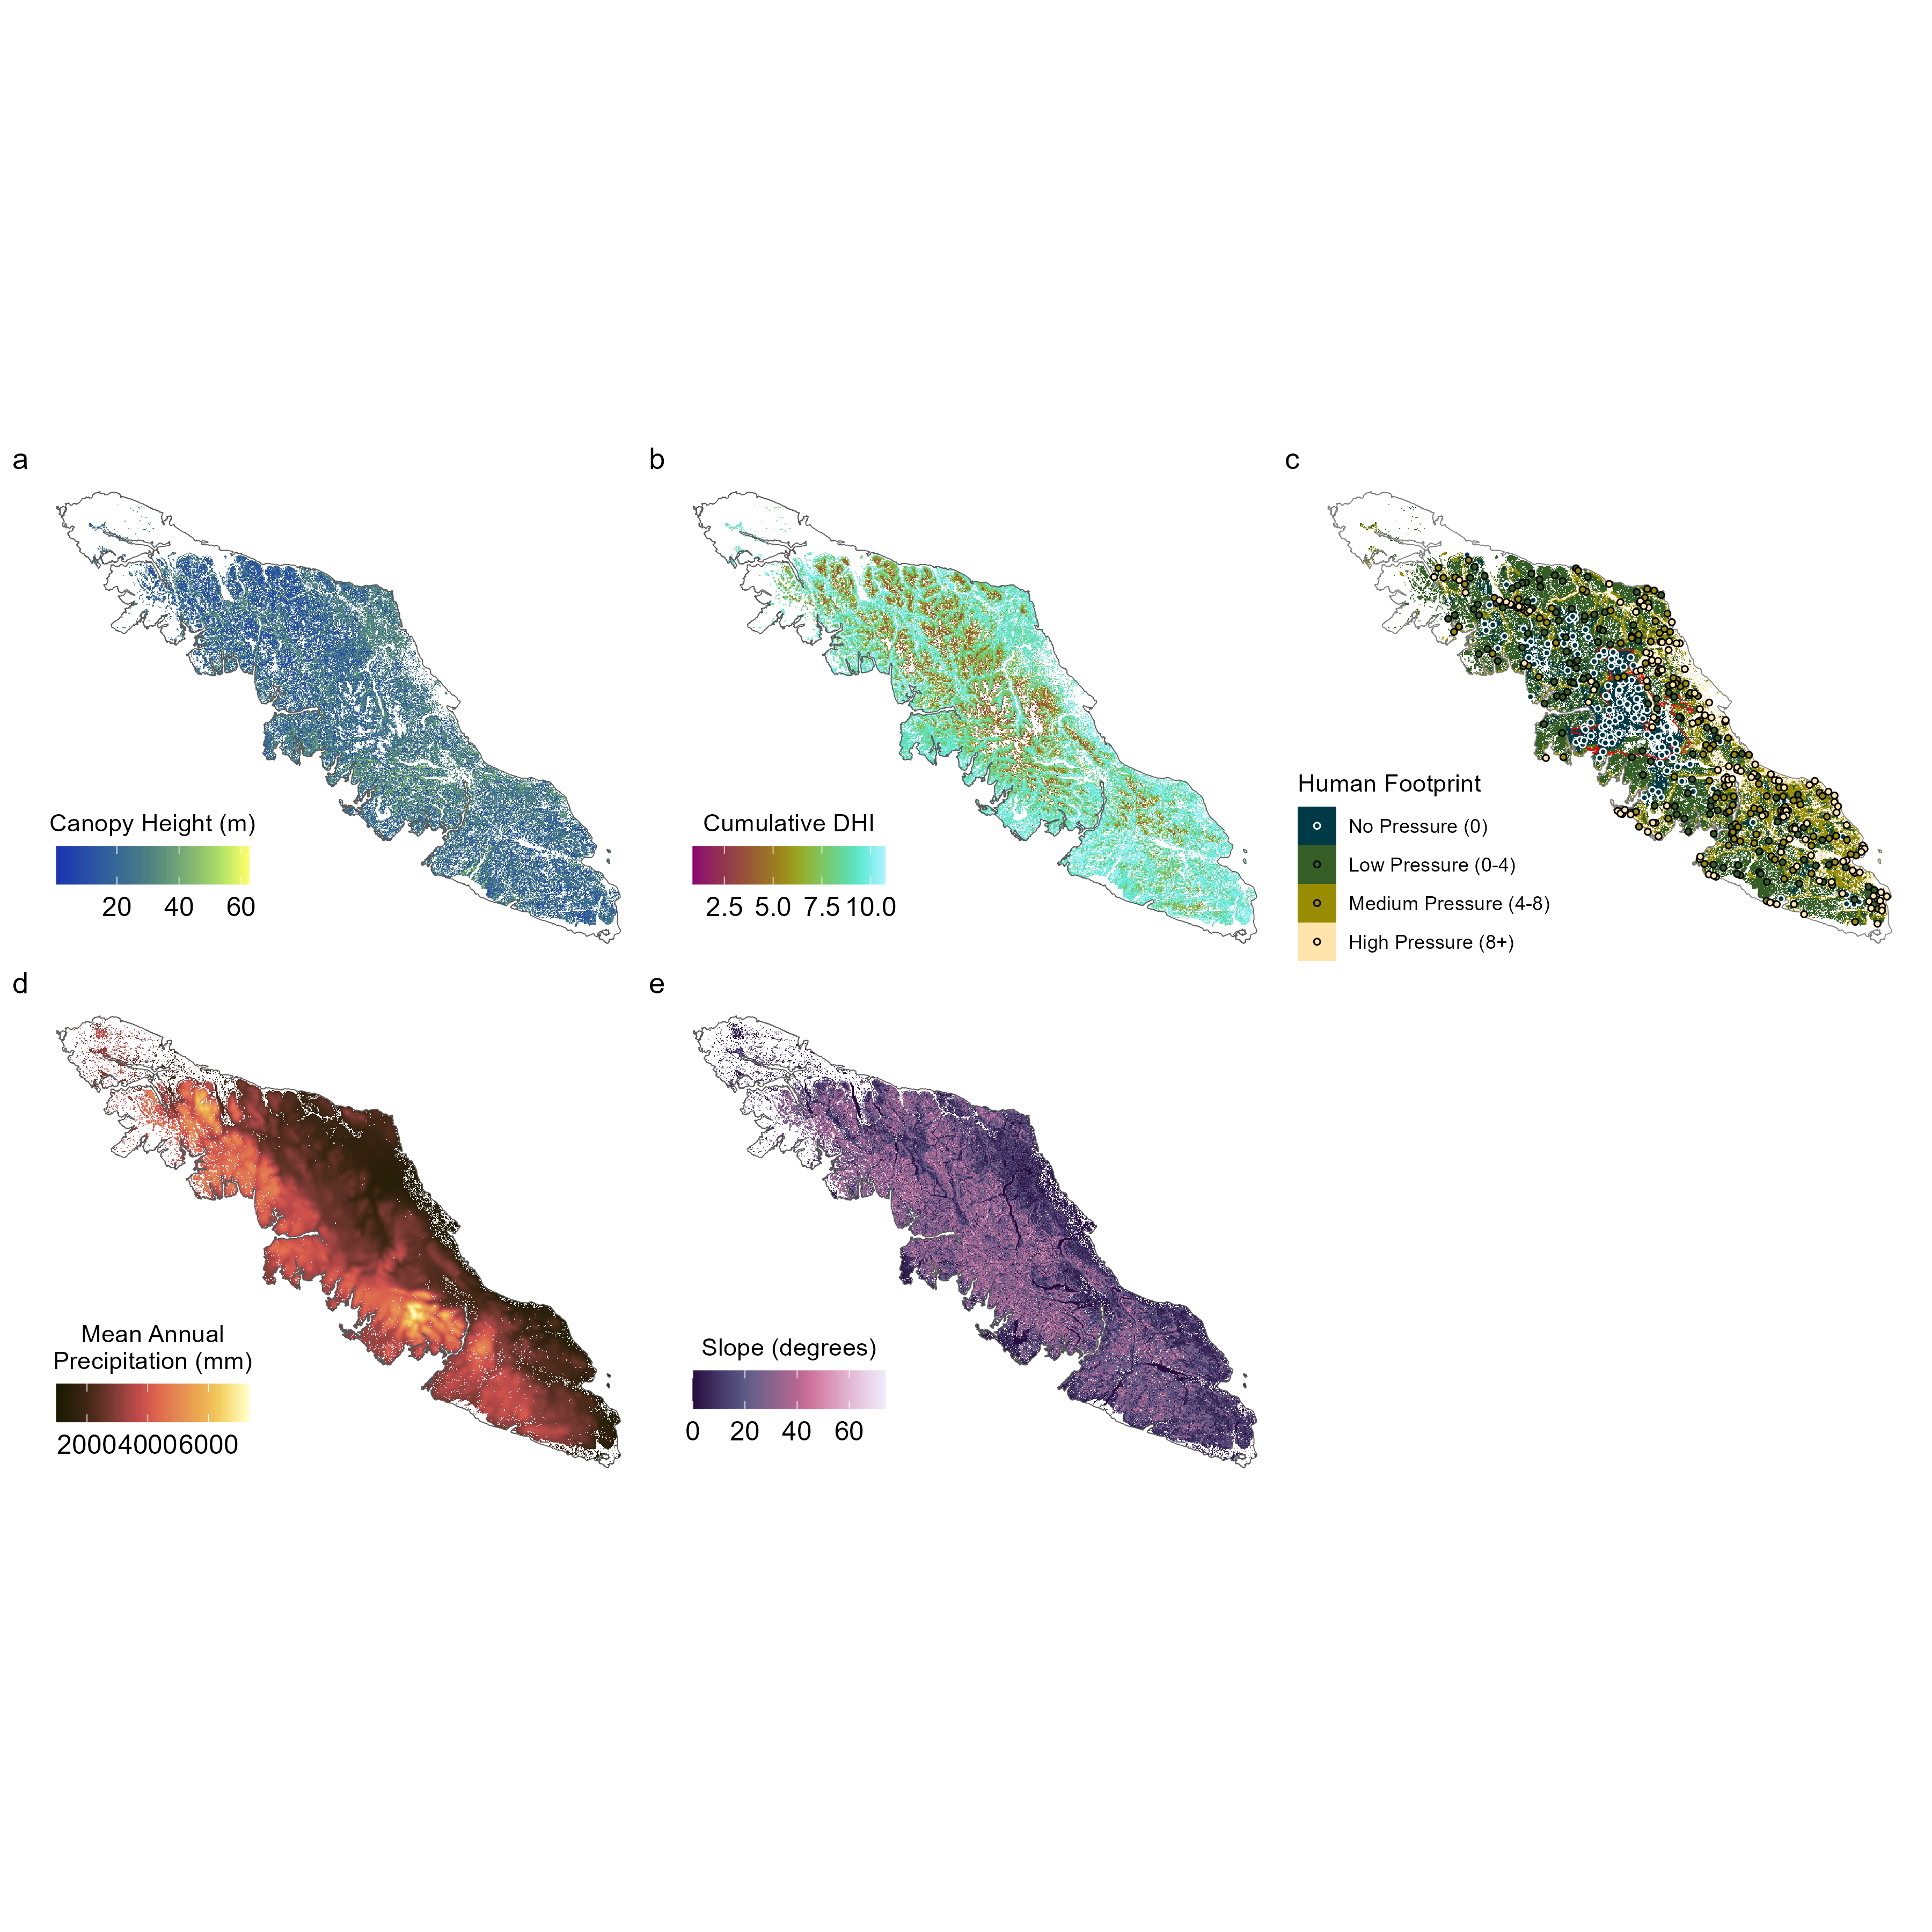
\includegraphics[width=12in,height=\textheight]{strathcona/figures/data_figure.png}

}

\caption{\label{fig-data}Visualization of the input datasets used in the
study. Panel C shows the human footprint and the location of the samples
used for our analysis.}

\end{figure}%

\subsection{Calculating similarity}\label{sec-sim}

We calculate the sigma dissimilarity (Mahony et al., 2017) of forested
pixels across British Columbia by using an expanded coarsened exact
matching (CEM) technique (Iacus et al., 2012) (Figure~\ref{fig-flow}).
This methodology enables us to evaluate the degree of similarity between
all forested pixels in the province and natural forests, while
accounting for potential confounding variables such as climate and
topography. The CEM technique creates comparable groups of observations
among covariates by initially coarsening the covariates. In this
instance, all six covariates were coarsened into five quintiles
hereafter referred to as bins. CEM then performs exact matching on the
bins, with each pixel matched to a climatically and topographically
similar group of pixels within Strathcona Park, hereafter referred to as
strata. In the case where there is not enough matched pixels found in
Strathcona Park, we calculate the nearest neighbours in bin space for
all strata, and sample up to 1000 pixels while minimizing the nearest
neighbour distance. If the nearest neighbour distance is on average
above two, we do not consider that strata in our analysis.

\phantomsection\label{cell-fig-flow}
\begin{figure}[H]

\centering{

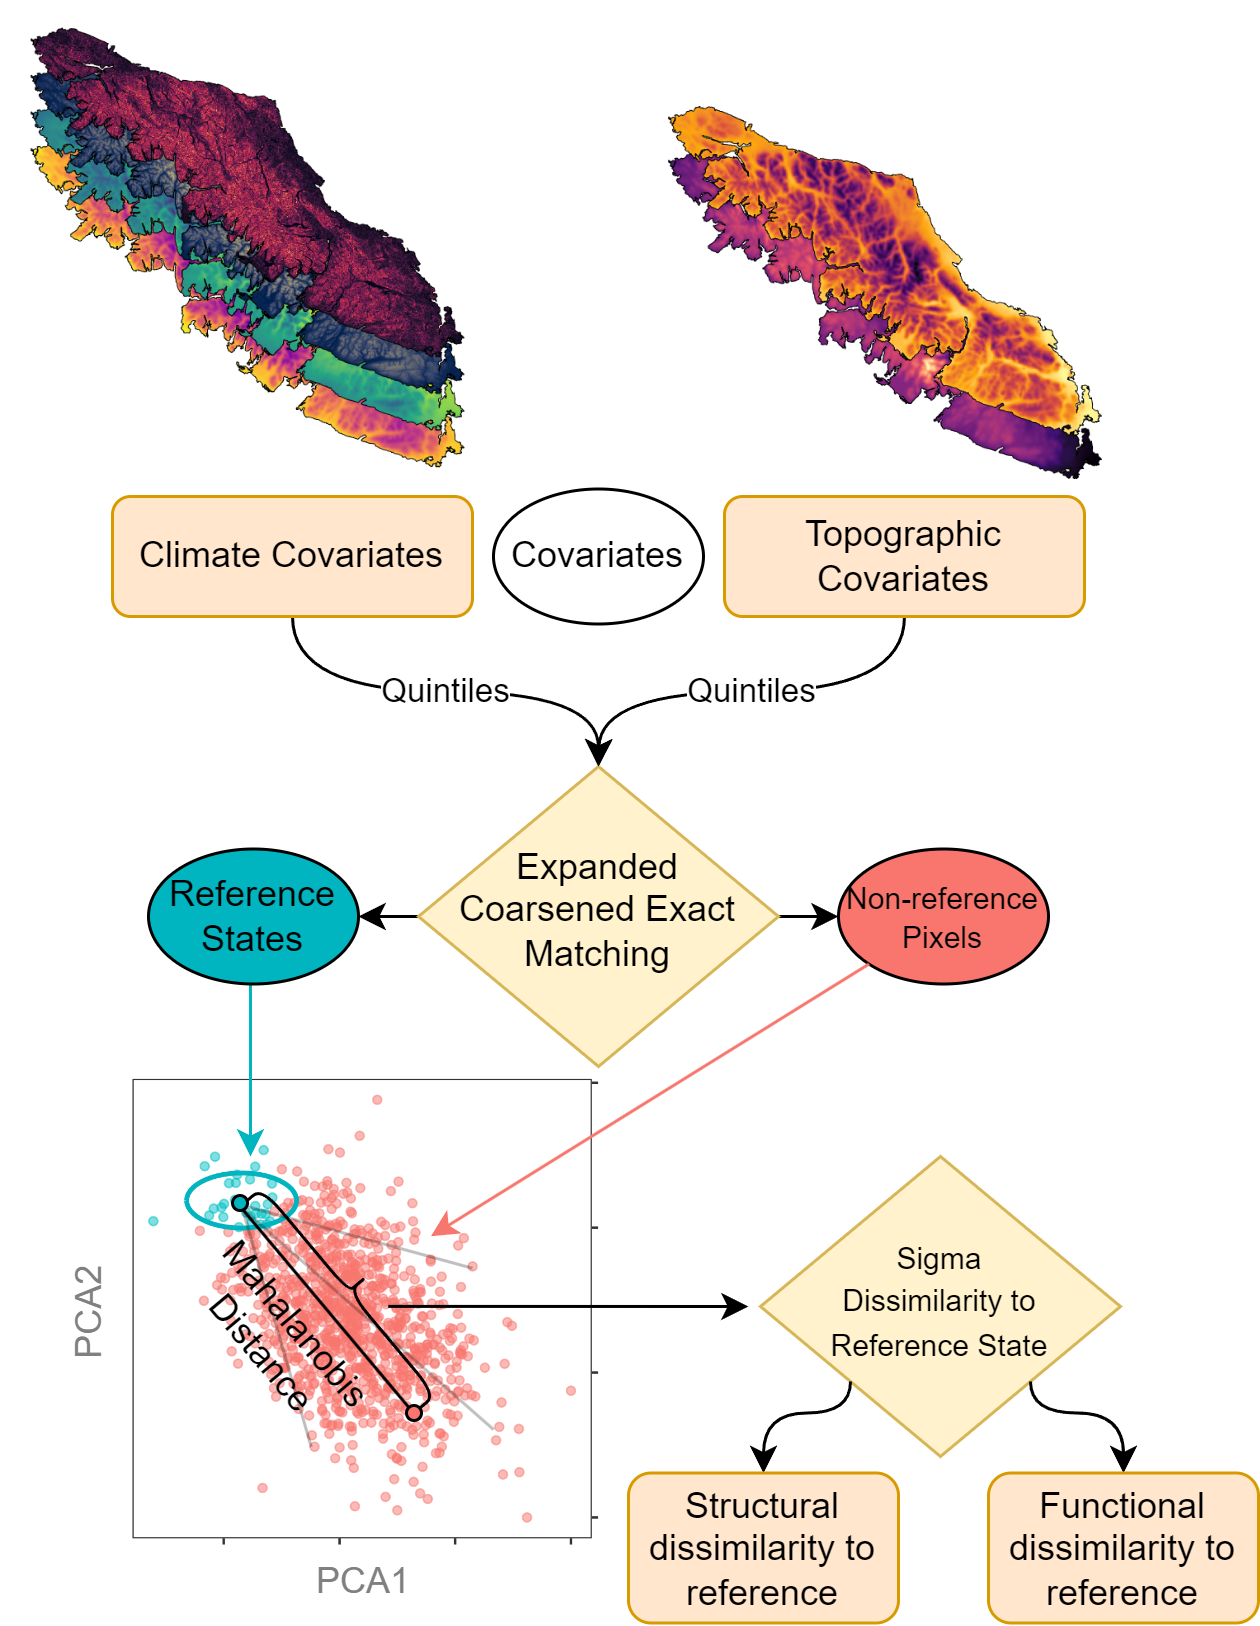
\includegraphics[width=5.25in,height=\textheight]{strathcona/figures/flow.drawio.png}

}

\caption{\label{fig-flow}Conceptual flow diagram of the study.}

\end{figure}%

Following the matching procedure, we identify data driven reference
states in both structural and functional attributes by selecting the top
10\% of protected, undisturbed observations for each structural (canopy
height, cover, and structural complexity) and functional (cumulative and
variation DHIs) attribute, separately. We then determine the similarity
of all pixels, in both structural and functional attributes, to the
reference states by calculating the sigma dissimilarity metric. Sigma
dissimilarity standardizes the Mahalanobian distance (Mahalanobis, 1936)
by rescaling it into percentiles of the chi distribution (Mahony et al.,
2017). This effectively accounts for the effect of dimensionality when
creating a multivariate similarity metric (Mahony et al., 2017). We
calculate sigma dissimilarity for every strata with a suitable reference
state, comparing all forested pixels to the top 10\% of each attribute
for that reference state.

\subsection{Sampling}\label{sampling}

We reclassify the Canadian Human Footprint (Hirsh-Pearson et al., n.d.;
Hirsh-Pearson et al., 2022) into categorical data following
Hirsh-Pearson et al. (2022) and Arias-Patino et al. (2024) : a value of
zero has no anthropogenic pressure, zero to four has low anthropogenic
pressure, four to eight has medium anthropogenic pressure, and
\textgreater{} eight has high anthropogenic pressure. To assess the
cumulative impact of anthropogenic pressure on ecological similarity, we
implement stratified sampling on all suitable strata, sampling 100
samples from each anthropogenic pressure class. For our individual
pressures, we follow the same reclassification steps on each pressure
layer, and sample an additional hundred samples for each pressure class.
Sampling was performed using the \textbf{sgsR} (version 1.4.5) R package
(Goodbody et al., 2023) with the Quiennec method (Queinnec et al.,
2021). Geospatial data processing was performed using the \textbf{terra}
(version 1.7-78) (Hijmans, 2024), \textbf{sf} (version 1.0-16) (Pebesma,
2018; Pebesma and Bivand, 2023), and \textbf{tidyterra} (version 0.6.1)
(Hernangómez, 2023a, 2023b) R packages.

\subsection{Analysis}\label{analysis}

We used a one-way analysis of variance (ANOVA) with a critical value of
0.05 to identify differences in the mean similarity values across
cumulative anthropogenic pressure classes. We account for family-wise
error rate for our ANOVAs using the Holm-Bonferroni method, only
continuing the analysis for similarity variables with significant ANOVAs
at the adjusted critical value. As ANOVAs only identify if there is a
difference in means, but does not identify which means are different, we
used a Tukey HSD post-hoc test to identify which means are different
from the control group (no anthropogenic pressure), which also controls
for the family-wise error rate.

We follow the same protocol to identify the difference in means for each
anthropogenic pressure of interest (roads, population density, forestry,
and built environment). We compare each pressure to the same `no
pressure' values sampled in the cumulative pressure analysis. All
statistical analysis were conducted using the \textbf{rstatix} (version
0.7.2) R package (Kassambara, 2023).

\section{Results}\label{results}

Our sigma dissimilarity processing workflow resulted in six island wide
maps of structural and functional similarity to the reference state
found in Strathcona Provincial Park (Figure~\ref{fig-regional}). We
display three selected subsets of Vancouver Island to demonstrate
variation in similarity and the anthorpogenic footprint layers. Subset A
shows a region near Lake Cowichan where harvesting is a common
anthropogenic pressure (Figure~\ref{fig-regional} A). Subset B shows a
protected area near Campbell River with high population density
(Figure~\ref{fig-regional} B). Subset C shows a region with generally
low anthropogenic pressure (Figure~\ref{fig-regional} C). We see more
variation in the similarity to high aboveground biomass and functional
reference states, while the similarity to canopy cover, canopy height,
and structural complexity is often lower across Vancouver Island.

\phantomsection\label{cell-fig-regional}
\begin{figure}[H]

\centering{

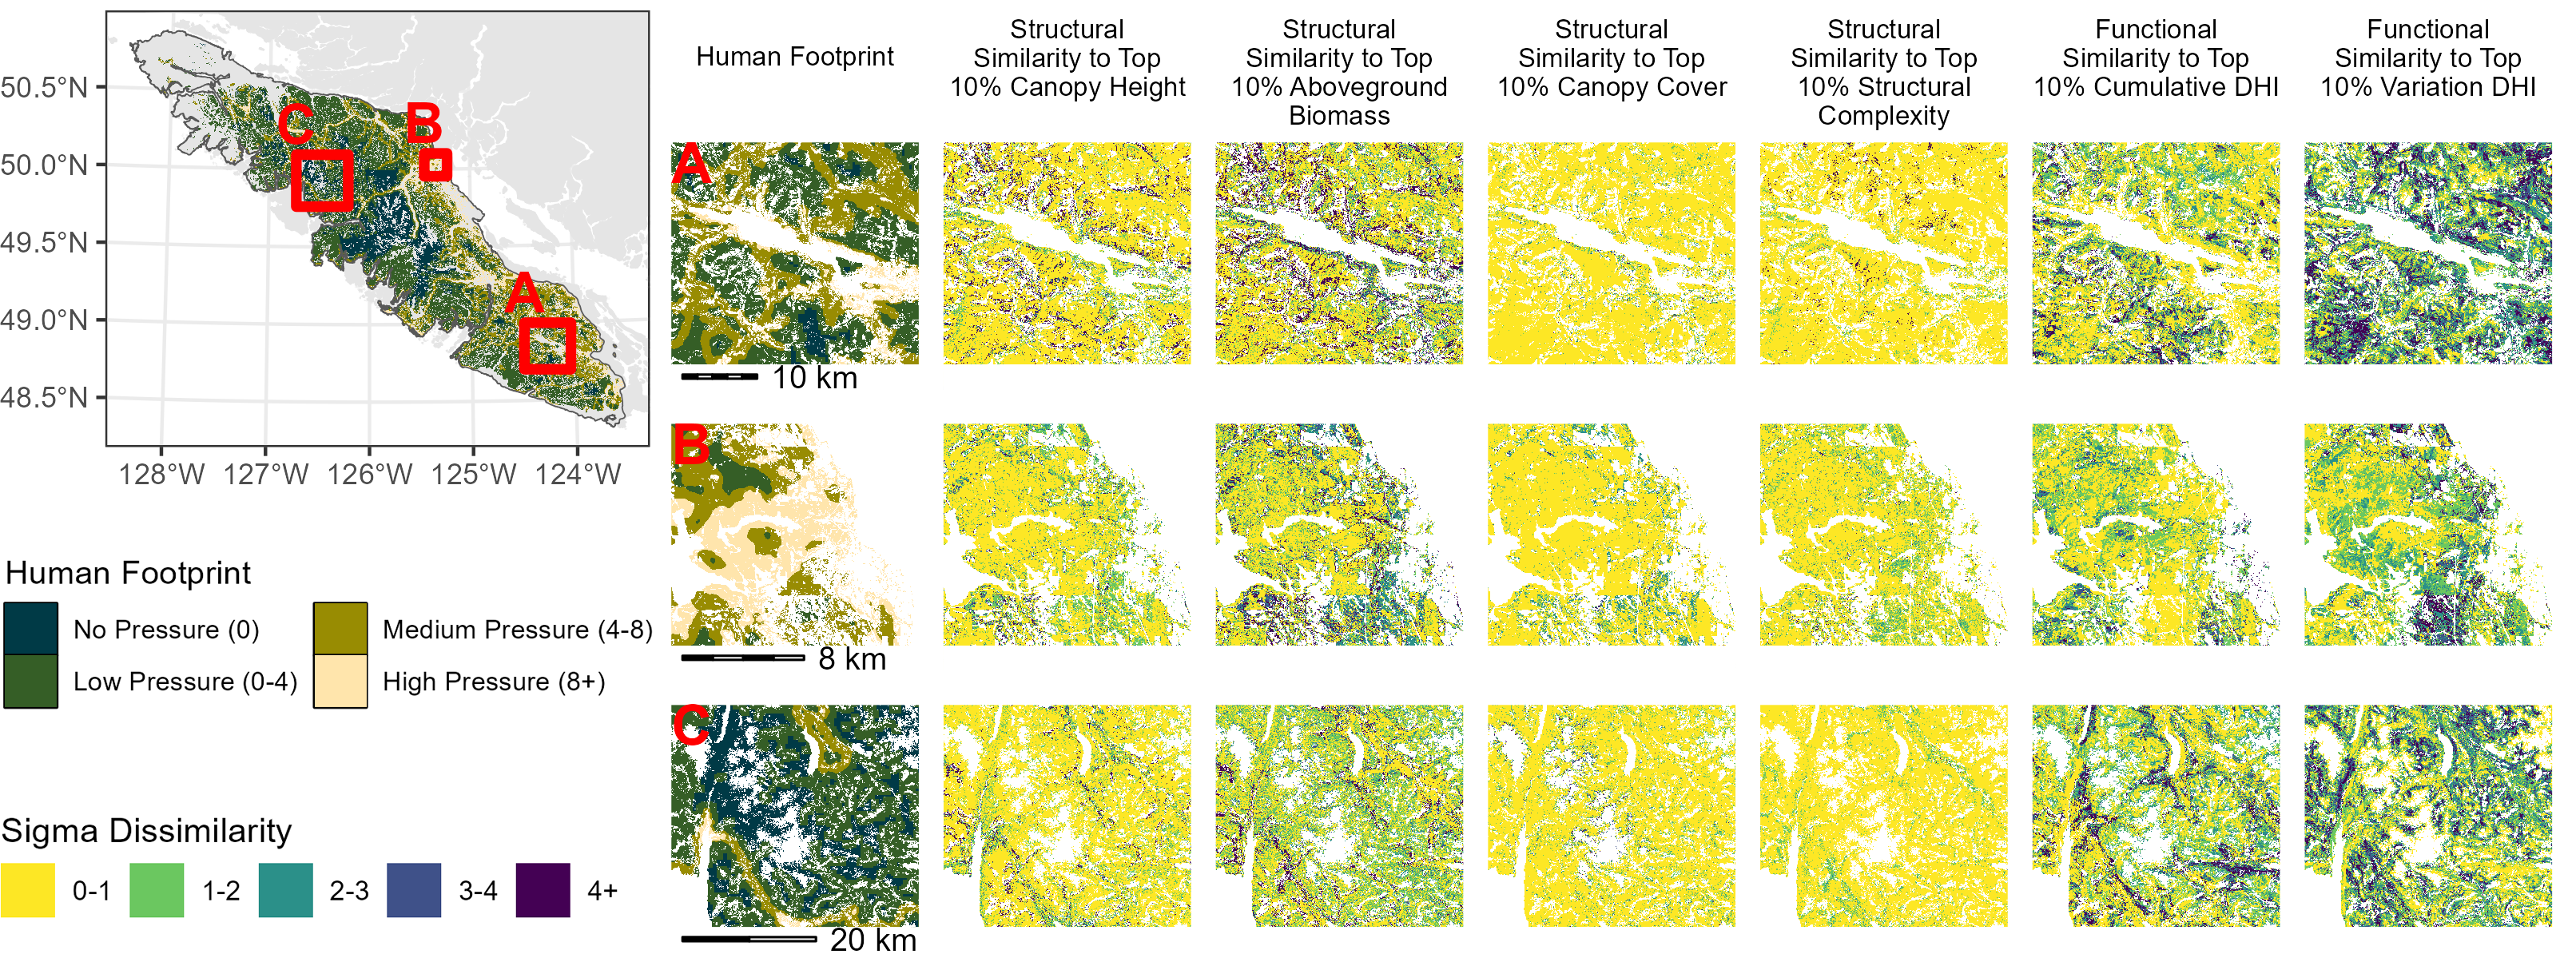
\includegraphics[width=10.75in,height=\textheight]{strathcona/figures/multi_panel_inset_wide_PS.png}

}

\caption{\label{fig-regional}Regional details of the human footprint and
sigma dissimilarity across the sites on Vancouver Island. Subset A show
Cowichan Lake, a heavily harvested region. Subset B shows Elk Falls
Provincial Park, just outside Campbell River, a region with high
population density. Subset C shows a region with generally low
anthropogenic pressure.}

\end{figure}%

We found that similarity to high structural complexity (Anova: p =
0.007) and tall canopy height (Anova: p = 0.003) reference states was
influenced by medium to high levels of cumulative anthropogenic pressure
(Figure~\ref{fig-boxplot-overall}). Similarity to high biomass (Anova: p
= 0.142) and canopy cover (Anova: p = 0.855) regions were not
significantly influenced by cumulative anthropogenic pressures. Neither
of the productivity metrics were influenced by cumulative anthropogenic
pressures.

\phantomsection\label{cell-fig-boxplot-overall}
\begin{figure}[H]

\centering{

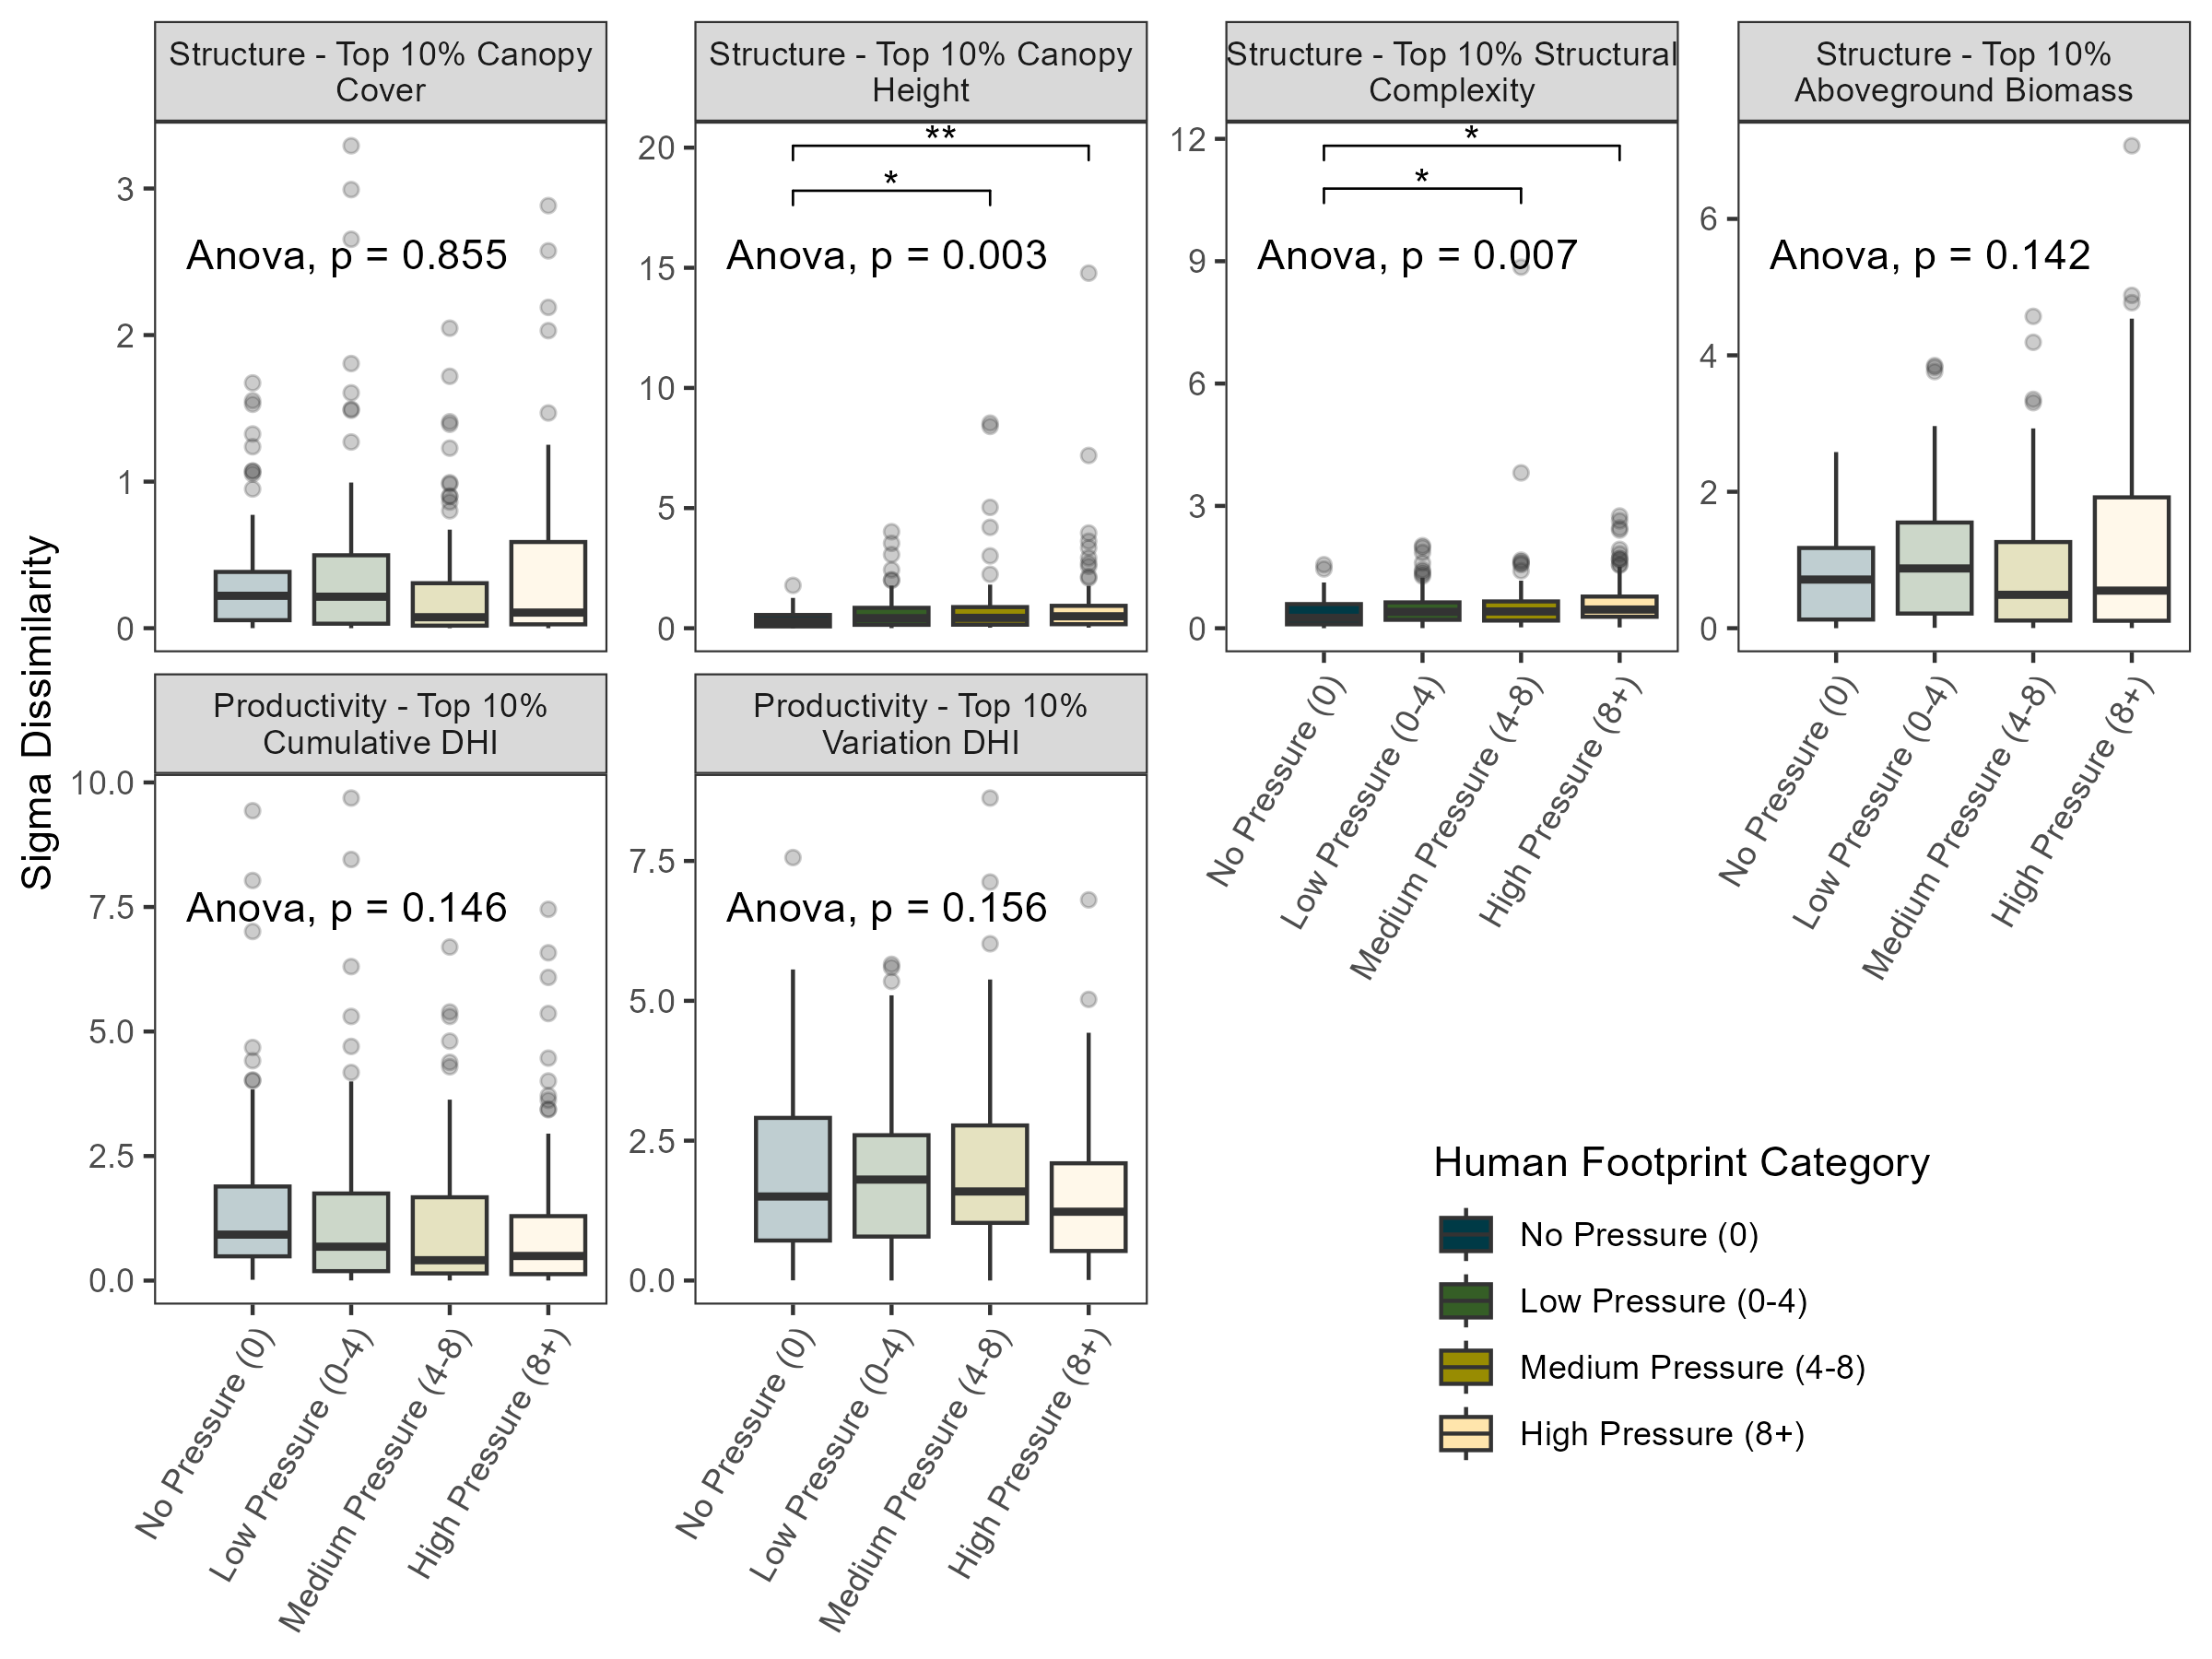
\includegraphics[width=8in,height=\textheight]{strathcona/figures/mahal_boxplot_sig.png}

}

\caption{\label{fig-boxplot-overall}Boxplots of sigma similarity to the
reference state in Strathcona Provincial Park by cumulative human
footprint category. Anova p-values corrected using the Holm-Bonferroni
method. * indicates a Tukey HSD p-value \textless{} 0.05. ** indicates a
Tukey HSD p-value \textless{} 0.01.}

\end{figure}%

Increases in all individual anthropogenic pressures led to increased
dissimilarity when compared to most structural reference states
(Figure~\ref{fig-boxplot-individual}). Increases in pressures from roads
and built environment did not increase or reduce similarity to
structural reference states with high canopy cover. Medium and high
pressures from population density and forestry/harvesting increased
dissimilarity to all structural reference states. Anthropogenic
pressures generally did not influence the similarity to reference states
based on productivity metrics, however, increases in pressures from
population density decreased dissimilarity to ecosystems with high
variation in energy availability.

\phantomsection\label{cell-fig-boxplot-individual}
\begin{figure}[H]

\centering{

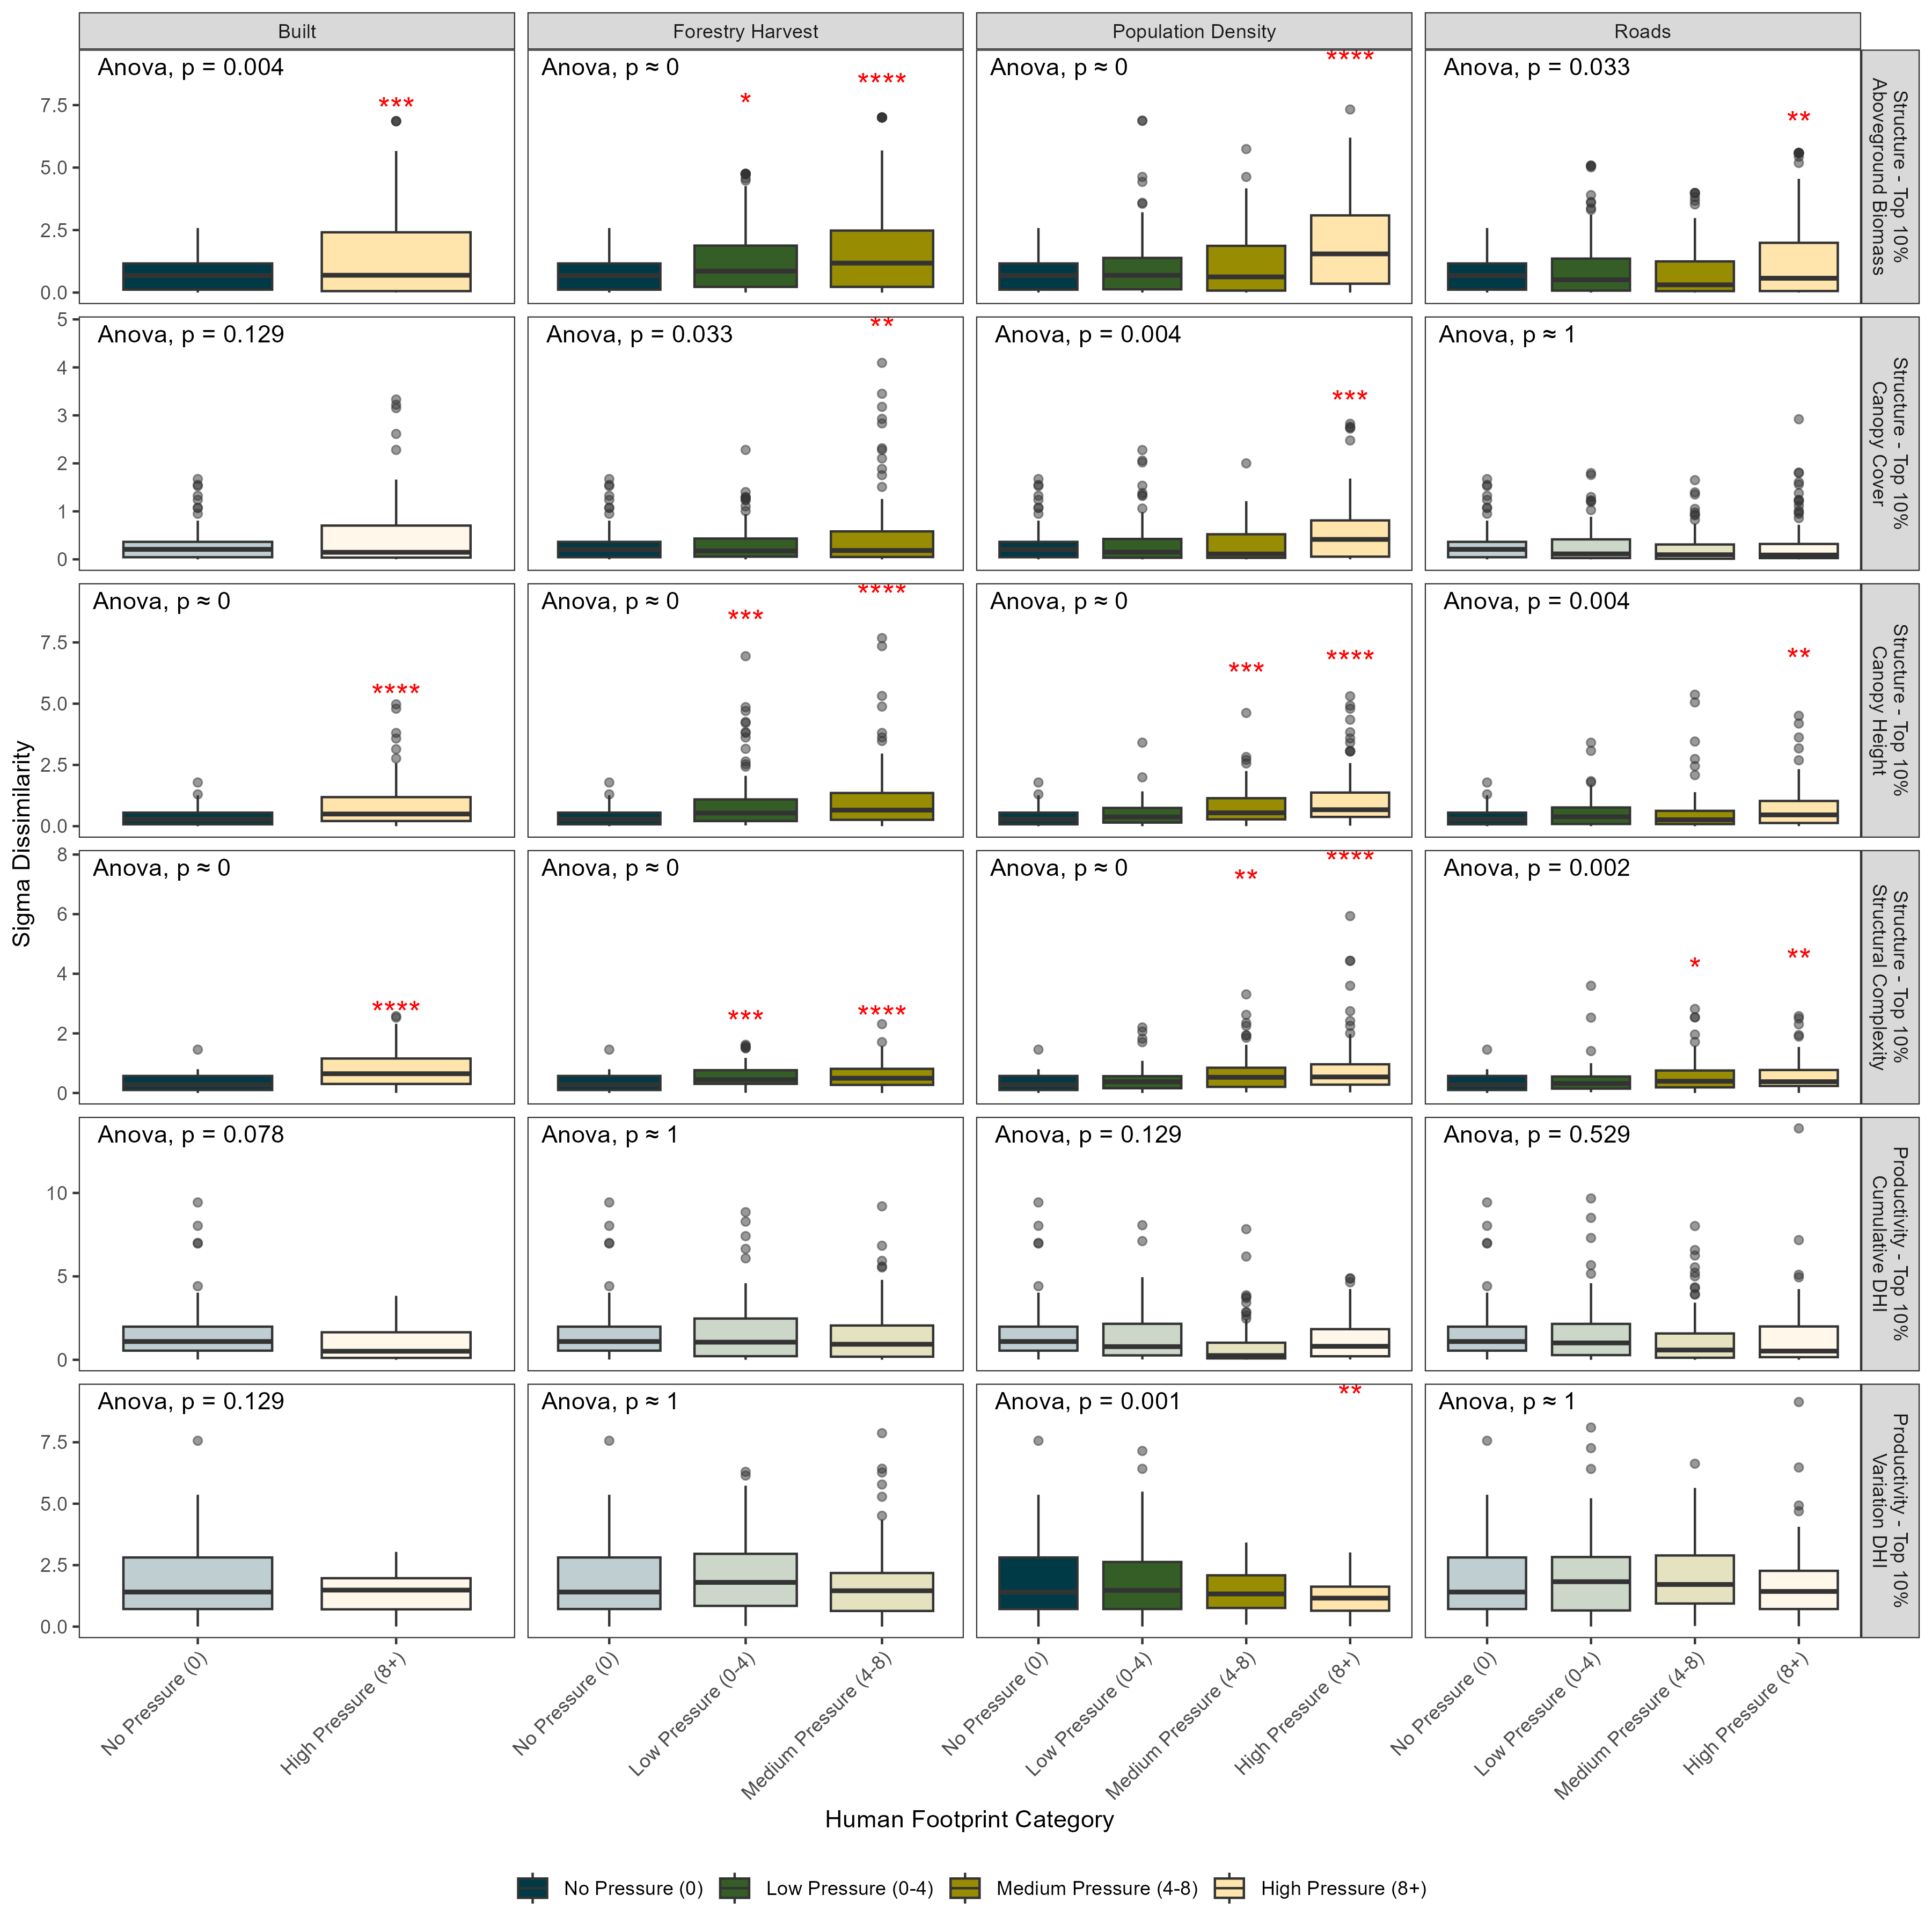
\includegraphics[width=8in,height=\textheight]{strathcona/figures/indiv_boxplots.png}

}

\caption{\label{fig-boxplot-individual}Boxplots of sigma similarity to
the reference state in Strathcona Provincial Park by individual
anthropogenic pressures. Anova p-values corrected using the
Holm-Bonferroni method. * indicates a Tukey HSD p-value \textless{}
0.05. ** indicates a Tukey HSD p-value \textless{} 0.01. *** indicates a
Tukey HSD p-value \textless{} 0.001. **** indicates a Tukey HSD p-value
\textless{} 0.0001.}

\end{figure}%

\section{Discussion}\label{discussion}

In this paper, we use medium-resolution remote sensing metrics of
ecosystem structure and function to assess similarity to high-integrity
forests across Vancouver Island, British Columbia. We validate our
approach by assessing the influence of the human footprint on these
reference states, finding that ecosystem structure in the form of forest
structural attributes is influenced by increased anthropogenic pressures
on a cumulative and individual level (Figure~\ref{fig-boxplot-overall};
Figure~\ref{fig-boxplot-individual}). Forest ecosystem function, as
represented by the DHIs, is generally not significantly influenced by
anthropogenic pressures, although population density increased
similarity to ecosystems with high variation in energy availability
(Figure~\ref{fig-boxplot-individual}).

We find that similarity to high structural complexity forests, which are
often high in biodiversity due to increased niche availability
(Macarthur and Macarthur, 1961; Walter et al., 2021), is impacted by
medium to high levels of anthropogenic pressures. Structural similarity
to tall forests is also impacted by medium to high levels of
anthropogenic pressure, while productivity metrics were not influenced
by cumulative anthropogenic pressures in this region
(Figure~\ref{fig-boxplot-overall}). In tropical forests, Bourgoin et al.
(2024) found that anthropogenic forest degradation influenced
aboveground biomass and canopy height, however, they focus on edge
effects, fire, and selective logging, rather than cumulative and
individual anthropogenic pressures. Li et al. (2023) also found a global
impact of anthropogenic pressures on forest structural density, however,
they do not explore which facets of anthropogenic pressure are the
strongest driver of forest degradation. Hansen et al. (2020) integrate
forest structure and anthropogenic pressure into the forest structural
integrity index to identify forest stands of high ecological value (high
structural quality; low anthropogenic footprint). We further this
research by assessing individual pressures on a multivariate metric of
structural similarity to a high-quality reference state
(Figure~\ref{fig-boxplot-individual}).

It is possible that we did not find a relationship between cumulative
anthropogenic pressures and canopy cover/aboveground biomass as these
forest structural attributes are typically high on Vancouver Island due
to the regions mild climate and suitability for forest growth (Waring et
al., 2006). Conversely, we did find a relationship between the vertical
layering (canopy height and structural complexity) of trees and
anthropogenic pressures (Figure~\ref{fig-boxplot-overall}). This is
especially relevant as structurally complex forests are crucial for
harbouring biodiversity and providing ecosystem functions and services.
The lack of a relationship between canopy cover/aboveground biomass and
the cumulative human footprint is potentially due to replanting efforts
from the forestry industry following harvest, which are required in
British Columbia and often lead to single species, single aged stands
(Lieffers et al., 2020). Stands of this configuration are unlikely to be
found in our reference state, Strathcona Provincial Park, as it has been
a protected area for over 100 years, thus leading to higher
dissimilarity values.

Anthropogenic effects on forest function and energy availability have
rarely been examined. Here, we also examine how anthropogenic pressures
influence similarity to high available energy and high energy variation
forests, both hypothesized to indicate high levels of biodiversity in a
number of guilds and clades (Radeloff et al., 2019; Razenkova et al.,
2022). We do not find a strong influence of cumulative anthropogenic
pressure on our forest functioning metrics, however, we did find that
similarity to forest stands with high annual energy variability was
increased in high population density areas
(Figure~\ref{fig-boxplot-individual}). This increase in similarity in
high density areas is potentially driven by ornamental trees and the
bias for North American urban forests to be primarily deciduous trees
(Clapp et al., 2014; Roman et al., 2018), which would have a stronger
variation DHI component due to annual leaf senescence and green-up.

Further, the calculation of the DHIs is dependent on using a vegetation
index or productivity estimate, in our case NDVI. Vegetation indices
have been shown to saturate at high levels of canopy cover and leaf area
index (Huete et al., 2002; Huete et al., 1997), which are common on
Vancouver Island, and comparisons of unprotected areas to the highest
10\% cover in reference states shows no significant difference
(Figure~\ref{fig-boxplot-overall}). Recent research has shown that
seasonality, here represented as the Variation DHI, drives functional
diversity in avian assemblages, however, these results also strongly
varied by region (Keyser et al., 2024). It is possible that examining
anthropogenic pressure impacts in regions with more variation in canopy
cover may lead to differing results depending on the amount of total
variation present in canopy cover, which would in turn influence
seasonality and energy availability.

Assessing individual pressure influences on the environment is also
relevant to questions of how cumulative anthropogenic pressure maps are
calculate. There is currently a debate between additive and antagonistic
anthropogenic pressure mapping methods, as there is little information
on mechanistic interactions between pressures (Arias-Patino et al.,
2024). We assess individual pressures on structural and functional
similarity in forests across Vancouver Island, Canada, an advancement
upon the current standard of using a single value of cumulative
anthropogenic pressure (Bourgoin et al., 2024; Li et al., 2023). Similar
methods could be used to examine mechanistic pressure interactions
across large scales.

We apply the Sigma Dissimilarity metric developed by Mahony et al.
(2017) to determine similarity to high-integrity ecosystems, and use a
matching approach to account for environmental covariates. This method
accounts for the multidimesnionality of the structure and function
datasets, and standardizes them so they are comparable. This is
especially relevant in our case as we use four forest structural
attributes and two forest function metrics. These methods are similar to
other similarity metrics commonly applied in remote sensing for
multivariate similarity such as spectral similarity (Schweiger et al.,
2018), and phenospectral similarity (Osei Darko et al., 2024).

While we are limited in number of structural variables due to the
imputation of the lidar-derived dataset across the study area (Matasci
et al., 2018a; Matasci et al., 2018b), future studies could directly use
raw lidar datasets to create a multitude of metrics, and apply the sigma
similarity method to those. This could capture additional facets of
similarity which are missed when using a Canada-wide dataset with
limited forest structural attributes at 30 m. New spaceborne lidar
missions such as GEDI (Dubayah et al., 2020) and IceSAT-II (Neumann et
al., 2019) are also providing estimates of forest structure across the
globe. However, these satellites are sample based missions, and do not
provide wall-to-wall coverage (Duncanson et al., 2021).

We assess multiple definitions of high quality forest across a large
region using a data-driven approach. Often, it is common for reference
states to be unavailable due to a lack of data on regions of high
ecological integrity, especially across large regions (McNellie et al.,
2020). We attempt to circumvent this by using a large, long-established
protected area (Strathcona Provincial Park; Figure~\ref{fig-study}), and
a matching technique that preserves ecological similarity between
reference states and their counterparts. The long-established, large
protected area ensures that little anthropogenic pressures or
modification have been made to the landscape, while also guaranteeing
that the reference state is attainable for a given topography and
climate (Corlett, 2016; Hobbs et al., 2014) due to contemporary nature
of the reference state. Our matching technique (coarsened exact
matching, combined with an kNN approach when no exact match is
available) allows us to generate reference states in a near wall-to-wall
fashion, which ensures similarity between reference state and compared
pixels.

Our techniques move beyond traditional impact evaluation techniques
(Ferraro, 2009) commonly used in protected area effectiveness
assessments by allowing spatial reconstruction of conservation outcomes,
and generating a multivariate, rather than univariate, assessment of
similarity to high ecological integrity forests. While our methods in
this paper use a data-driven approach to derive reference states, if an
individual or organization is interested in a specific species or
ecosystem, and has known locations of high quality ecosystems associated
with that species or ecosystem, these methods can be applied to assess
similarity to those high quality ecosystems across large regions.

\section{Acknowledgements}\label{acknowledgements}

This research was funded by NSERC support of Coops (RGPIN-2024-04402).
Remote sensing data products used in this research are free and open and
available for download at \url{https://ca.nfis.org/maps_eng.html}. The
authors thank Dr.~Michael A. Wulder and Dr.~Joanne C. White for
development and early access to these National Terrestrial Ecosystem
Mapping System (NTEMS) products. They thank Dr.~Elena Razenkova for
early access to the Landsat-derived Dynamic Habitat Indices. ERM would
like to thank the members of the IRSS for many helpful conversations
throughout the preparation of this manuscript.

\section{Ethics}\label{ethics}

The authors declare no conflicts of interest.

\section*{References}\label{references}
\addcontentsline{toc}{section}{References}

\phantomsection\label{refs}
\begin{CSLReferences}{1}{0}
\vspace{1em}

\bibitem[\citeproctext]{ref-andrew2012}
Andrew, M.E., Wulder, M.A., Coops, N.C., 2012. Identification of
{\emph{de facto}} protected areas in boreal canada. Biological
Conservation 146, 97--107.
\url{https://doi.org/10.1016/j.biocon.2011.11.029}

\bibitem[\citeproctext]{ref-arcese1997}
Arcese, P., Sinclair, A.R.E., 1997. The role of protected areas as
ecological baselines. The Journal of Wildlife Management 61, 587--602.
\url{https://doi.org/10.2307/3802167}

\bibitem[\citeproctext]{ref-arias-patino2024}
Arias-Patino, M., Johnson, C.J., Schuster, R., Wheate, R.D., Venter, O.,
2024. Accuracy, uncertainty, and biases in cumulative pressure mapping.
Ecological Indicators 166, 112407.
\url{https://doi.org/10.1016/j.ecolind.2024.112407}

\bibitem[\citeproctext]{ref-balaguer2014}
Balaguer, L., Escudero, A., Martín-Duque, J.F., Mola, I., Aronson, J.,
2014. The historical reference in restoration ecology: Re-defining a
cornerstone concept. Biological Conservation 176, 12--20.
\url{https://doi.org/10.1016/j.biocon.2014.05.007}

\bibitem[\citeproctext]{ref-becker2023}
Becker, A., Russo, S., Puliti, S., Lang, N., Schindler, K., Wegner,
J.D., 2023. Country-wide retrieval of forest structure from optical and
SAR satellite imagery with deep ensembles. ISPRS Journal of
Photogrammetry and Remote Sensing 195, 269--286.
\url{https://doi.org/10.1016/j.isprsjprs.2022.11.011}

\bibitem[\citeproctext]{ref-bourgoin2024}
Bourgoin, C., Ceccherini, G., Girardello, M., Vancutsem, C., Avitabile,
V., Beck, P.S.A., Beuchle, R., Blanc, L., Duveiller, G., Migliavacca,
M., Vieilledent, G., Cescatti, A., Achard, F., 2024. Human degradation
of tropical moist forests is greater than previously estimated. Nature
631, 570--576. \url{https://doi.org/10.1038/s41586-024-07629-0}

\bibitem[\citeproctext]{ref-brumelis2011}
Brumelis, G., Jonsson, B.G., Kouki, J., Kuuluvainen, T., Shorohova, E.,
2011. \href{https://www.silvafennica.fi/article/446}{Forest naturalness
in northern Europe: perspectives on processes, structures and species
diversity}. Silva Fennica 45.

\bibitem[\citeproctext]{ref-burns1990}
Burns, R.M., 1990. Silvics of North America. U.S. Department of
Agriculture, Forest Service.

\bibitem[\citeproctext]{ref-cardinale2012}
Cardinale, B.J., Duffy, J.E., Gonzalez, A., Hooper, D.U., Perrings, C.,
Venail, P., Narwani, A., Mace, G.M., Tilman, D., Wardle, D.A., Kinzig,
A.P., Daily, G.C., Loreau, M., Grace, J.B., Larigauderie, A.,
Srivastava, D.S., Naeem, S., 2012. Biodiversity loss and its impact on
humanity. Nature 486, 59--67. \url{https://doi.org/10.1038/nature11148}

\bibitem[\citeproctext]{ref-clapp2014}
Clapp, J.C., Ryan III, H.D.P., Harper, R.W., Bloniarz, D.V., 2014.
Rationale for the increased use of conifers as functional green
infrastructure: A literature review and synthesis. Arboricultural
Journal 36, 161--178. \url{https://doi.org/10.1080/03071375.2014.950861}

\bibitem[\citeproctext]{ref-reporto2023}
Convention on Biological Diversity, 2023. Report of the conference of
the parties to the {Convention} on {Biological Diversity} on the second
part of its fifteenth meeting (No. CBD/COP/15/17).

\bibitem[\citeproctext]{ref-coops2019}
Coops, N.C., Bolton, D.K., Hobi, M.L., Radeloff, V.C., 2019. Untangling
multiple species richness hypothesis globally using remote sensing
habitat indices. Ecological Indicators 107.
\url{https://doi.org/10.1016/j.ecolind.2019.105567}

\bibitem[\citeproctext]{ref-WOS:000265076300011}
Coops, N.C., Waring, R.H., Wulder, M.A., Pidgeon, A.M., Radeloff, V.C.,
2009. Bird diversity: A predictable function of satellite-derived
estimates of seasonal variation in canopy light absorbance across the
united states. JOURNAL OF BIOGEOGRAPHY 36, 905--918.
\url{https://doi.org/10.1111/j.1365-2699.2008.02053.x}

\bibitem[\citeproctext]{ref-corlett2016}
Corlett, R.T., 2016. Restoration, reintroduction, and rewilding in a
changing world. Trends in Ecology \& Evolution 31, 453--462.
\url{https://doi.org/10.1016/j.tree.2016.02.017}

\bibitem[\citeproctext]{ref-daniels2006}
Daniels, L.D., Gray, R.W., 2006. Disturbance regimes in coastal British
Columbia. Journal of Ecosystems and Management 7.
\url{https://doi.org/10.22230/jem.2006v7n2a542}

\bibitem[\citeproctext]{ref-dirzo2003}
Dirzo, R., Raven, P.H., 2003. Global State of Biodiversity and Loss.
Annual Review of Environment and Resources 28, 137--167.
\url{https://doi.org/10.1146/annurev.energy.28.050302.105532}

\bibitem[\citeproctext]{ref-dubayah2020}
Dubayah, R., Blair, J.B., Goetz, S., Fatoyinbo, L., Hansen, M., Healey,
S., Hofton, M., Hurtt, G., Kellner, J., Luthcke, S., Armston, J., Tang,
H., Duncanson, L., Hancock, S., Jantz, P., Marselis, S., Patterson,
P.L., Qi, W., Silva, C., 2020. The Global Ecosystem Dynamics
Investigation: High-resolution laser ranging of the Earth{'}s forests
and topography. Science of Remote Sensing 1, 100002.
\url{https://doi.org/10.1016/j.srs.2020.100002}

\bibitem[\citeproctext]{ref-duncanson2021}
Duncanson, L., Neuenschwander, A., Silva, C.A., Montesano, P., Guenther,
E., Thomas, N., Hancock, S., Minor, D., White, J., Wulder, M., Armston,
J., 2021. 2021 IEEE international geoscience and remote sensing
symposium IGARSS. pp. 670--672.
\url{https://doi.org/10.1109/IGARSS47720.2021.9553209}

\bibitem[\citeproctext]{ref-ferraro2009}
Ferraro, P.J., 2009. Counterfactual thinking and impact evaluation in
environmental policy. New Directions for Evaluation 2009, 75--84.
\url{https://doi.org/10.1002/ev.297}

\bibitem[\citeproctext]{ref-goodbody2023}
Goodbody, T.R.H., Coops, N.C., Queinnec, M., White, J.C., Tompalski, P.,
Hudak, A.T., Auty, D., Valbuena, R., LeBoeuf, A., Sinclair, I.,
McCartney, G., Prieur, J.-F., Woods, M.E., 2023. sgsR: A structurally
guided sampling toolbox for LiDAR-based forest inventories. Forestry: An
International Journal of Forest Research cpac055.
\url{https://doi.org/10.1093/forestry/cpac055}

\bibitem[\citeproctext]{ref-gorelick2017}
Gorelick, N., Hancher, M., Dixon, M., Ilyushchenko, S., Thau, D., Moore,
R., 2017. Google Earth Engine: Planetary-scale geospatial analysis for
everyone. Remote Sensing of Environment, Big Remotely Sensed Data:
tools, applications and experiences 202, 18--27.
\url{https://doi.org/10.1016/j.rse.2017.06.031}

\bibitem[\citeproctext]{ref-grantham2020}
Grantham, H.S., Duncan, A., Evans, T.D., Jones, K.R., Beyer, H.L.,
Schuster, R., Walston, J., Ray, J.C., Robinson, J.G., Callow, M.,
Clements, T., Costa, H.M., DeGemmis, A., Elsen, P.R., Ervin, J., Franco,
P., Goldman, E., Goetz, S., Hansen, A., Hofsvang, E., Jantz, P.,
Jupiter, S., Kang, A., Langhammer, P., Laurance, W.F., Lieberman, S.,
Linkie, M., Malhi, Y., Maxwell, S., Mendez, M., Mittermeier, R., Murray,
N.J., Possingham, H., Radachowsky, J., Saatchi, S., Samper, C.,
Silverman, J., Shapiro, A., Strassburg, B., Stevens, T., Stokes, E.,
Taylor, R., Tear, T., Tizard, R., Venter, O., Visconti, P., Wang, S.,
Watson, J.E.M., 2020. Anthropogenic modification of forests means only
40. Nature Communications 11, 5978.
\url{https://doi.org/10.1038/s41467-020-19493-3}

\bibitem[\citeproctext]{ref-hansen2019}
Hansen, A., Barnett, K., Jantz, P., Phillips, L., Goetz, S.J., Hansen,
M., Venter, O., Watson, J.E.M., Burns, P., Atkinson, S.,
Rodríguez-Buritica, S., Ervin, J., Virnig, A., Supples, C., De Camargo,
R., 2019. Global humid tropics forest structural condition and forest
structural integrity maps. Scientific Data 6, 232.
\url{https://doi.org/10.1038/s41597-019-0214-3}

\bibitem[\citeproctext]{ref-hansen2020}
Hansen, A.J., Burns, P., Ervin, J., Goetz, S.J., Hansen, M., Venter, O.,
Watson, J.E.M., Jantz, P.A., Virnig, A.L.S., Barnett, K., Pillay, R.,
Atkinson, S., Supples, C., Rodríguez-Buritica, S., Armenteras, D., 2020.
A policy-driven framework for conserving the best of Earth{'}s remaining
moist tropical forests. Nature Ecology \& Evolution 4, 1377--1384.
\url{https://doi.org/10.1038/s41559-020-1274-7}

\bibitem[\citeproctext]{ref-hansen2021}
Hansen, A.J., Noble, B.P., Veneros, J., East, A., Goetz, S.J., Supples,
C., Watson, J.E.M., Jantz, P.A., Pillay, R., Jetz, W., Ferrier, S.,
Grantham, H.S., Evans, T.D., Ervin, J., Venter, O., Virnig, A.L.S.,
2021. Toward monitoring forest ecosystem integrity within the post-2020
Global Biodiversity Framework. Conservation Letters 14, e12822.
\url{https://doi.org/10.1111/conl.12822}

\bibitem[\citeproctext]{ref-harfoot2018}
Harfoot, M.B.J., Tittensor, D.P., Knight, S., Arnell, A.P., Blyth, S.,
Brooks, S., Butchart, S.H.M., Hutton, J., Jones, M.I., Kapos, V.,
Scharlemann, J.P.W., Burgess, N.D., 2018. Present and future
biodiversity risks from fossil fuel exploitation. Conservation Letters
11, e12448. \url{https://doi.org/10.1111/conl.12448}

\bibitem[\citeproctext]{ref-hedwall2019}
Hedwall, P.-O., Gustafsson, L., Brunet, J., Lindbladh, M., Axelsson,
A.-L., Strengbom, J., 2019. Half a century of multiple anthropogenic
stressors has altered northern forest understory plant communities.
ECOLOGICAL APPLICATIONS 29, e01874.
\url{https://doi.org/10.1002/eap.1874}

\bibitem[\citeproctext]{ref-hermosilla2015}
Hermosilla, T., Wulder, M.A., White, J.C., Coops, N.C., Hobart, G.W.,
2015. An integrated landsat time series protocol for change detection
and generation of annual gap-free surface reflectance composites. Remote
Sensing of Environment 158, 220234.
\url{https://doi.org/10.1016/j.rse.2014.11.005}

\bibitem[\citeproctext]{ref-hermosilla2016}
Hermosilla, T., Wulder, M.A., White, J.C., Coops, N.C., Hobart, G.W.,
Campbell, L.B., 2016. Mass data processing of time series landsat
imagery: Pixels to data products for forest monitoring. International
Journal of Digital Earth 9, 10351054.
\url{https://doi.org/10.1080/17538947.2016.1187673}

\bibitem[\citeproctext]{ref-hernanguxf3mez2023}
Hernangómez, D., 2023a. Using the tidyverse with terra objects: the
tidyterra package. Journal of Open Source Software 8, 5751.
\url{https://doi.org/10.21105/joss.05751}

\bibitem[\citeproctext]{ref-R-tidyterra}
Hernangómez, D., 2023b. Using the {tidyverse} with {terra} objects: The
{tidyterra} package. Journal of Open Source Software 8, 5751.
\url{https://doi.org/10.21105/joss.05751}

\bibitem[\citeproctext]{ref-R-terra}
Hijmans, R.J., 2024. \href{https://rspatial.org/}{Terra: Spatial data
analysis}.

\bibitem[\citeproctext]{ref-hirsh-pearson2022}
Hirsh-Pearson, K., Johnson, C.J., Schuster, R., Wheate, R.D., Venter,
O., 2022. Canada{'}s human footprint reveals large intact areas
juxtaposed against areas under immense anthropogenic pressure. FACETS 7,
398--419. \url{https://doi.org/10.1139/facets-2021-0063}

\bibitem[\citeproctext]{ref-hirsh-pearson}
Hirsh-Pearson, K., Johnson, C., Schuster, R., Wheate, R., Venter, O.,
n.d. The Canadian Human Footprint.
\url{https://doi.org/10.5683/SP2/EVKAVL}

\bibitem[\citeproctext]{ref-hobbs2014}
Hobbs, R.J., Higgs, E., Hall, C.M., Bridgewater, P., Chapin III, F.S.,
Ellis, E.C., Ewel, J.J., Hallett, L.M., Harris, J., Hulvey, K.B.,
Jackson, S.T., Kennedy, P.L., Kueffer, C., Lach, L., Lantz, T.C., Lugo,
A.E., Mascaro, J., Murphy, S.D., Nelson, C.R., Perring, M.P.,
Richardson, D.M., Seastedt, T.R., Standish, R.J., Starzomski, B.M.,
Suding, K.N., Tognetti, P.M., Yakob, L., Yung, L., 2014. Managing the
whole landscape: historical, hybrid, and novel ecosystems. Frontiers in
Ecology and the Environment 12, 557--564.
\url{https://doi.org/10.1890/130300}

\bibitem[\citeproctext]{ref-huete2002}
Huete, A., Didan, K., Miura, T., Rodriguez, E.P., Gao, X., Ferreira,
L.G., 2002. Overview of the radiometric and biophysical performance of
the MODIS vegetation indices. Remote Sensing of Environment 83,
195--213. \url{https://doi.org/10.1016/S0034-4257(02)00096-2}

\bibitem[\citeproctext]{ref-huete1997}
Huete, A.R., Liu, H., Leeuwen, W.J.D. van, 1997. IGARSS'97. 1997 IEEE
international geoscience and remote sensing symposium proceedings.
Remote sensing - a scientific vision for sustainable development. pp.
1966--1968 vol.4. \url{https://doi.org/10.1109/IGARSS.1997.609169}

\bibitem[\citeproctext]{ref-iacus2012}
Iacus, S.M., King, G., Porro, G., 2012. Causal Inference without Balance
Checking: Coarsened Exact Matching. Political Analysis 20, 1--24.
\url{https://doi.org/10.1093/pan/mpr013}

\bibitem[\citeproctext]{ref-joppa2009}
Joppa, L.N., Pfaff, A., 2009. High and Far: Biases in the Location of
Protected Areas. PLOS ONE 4, e8273.
\url{https://doi.org/10.1371/journal.pone.0008273}

\bibitem[\citeproctext]{ref-R-rstatix}
Kassambara, A., 2023.
\href{https://rpkgs.datanovia.com/rstatix/}{Rstatix: Pipe-friendly
framework for basic statistical tests}.

\bibitem[\citeproctext]{ref-keyser2024}
Keyser, S.R., Pauli, J.N., Fink, D., Radeloff, V.C., Pigot, A.L.,
Zuckerberg, B., 2024. Seasonality Structures Avian Functional Diversity
and Niche Packing Across North America. Ecology Letters 27, e14521.
\url{https://doi.org/10.1111/ele.14521}

\bibitem[\citeproctext]{ref-li2023}
Li, W., Guo, W.-Y., Pasgaard, M., Niu, Z., Wang, L., Chen, F., Qin, Y.,
Svenning, J.-C., 2023. Human fingerprint on structural density of
forests globally. Nature Sustainability 6, 368--379.
\url{https://doi.org/10.1038/s41893-022-01020-5}

\bibitem[\citeproctext]{ref-lieffers2020}
Lieffers, V.J., Pinno, B.D., Beverly, J.L., Thomas, B.R., Nock, C.,
2020. Reforestation policy has constrained options for managing risks on
public forests. Canadian Journal of Forest Research 50, 855--861.
\url{https://doi.org/10.1139/cjfr-2019-0422}

\bibitem[\citeproctext]{ref-liira2007}
Liira, J., Sepp, T., Parrest, O., 2007. The forest structure and
ecosystem quality in conditions of anthropogenic disturbance along
productivity gradient. Forest Ecology and Management, Disturbances at
multiple scales as the basis of forest ecosystem restoration and
management 250, 34--46.
\url{https://doi.org/10.1016/j.foreco.2007.03.007}

\bibitem[\citeproctext]{ref-macarthur1961}
Macarthur, R., Macarthur, J., 1961. On bird species-diversity. Ecology
42, 594-- \&. \url{https://doi.org/10.2307/1932254}

\bibitem[\citeproctext]{ref-mahalanobis1936generalized}
Mahalanobis, P.C., 1936. On the generalized distance in statistics.
Proceedings of the National Institute of Sciences (Calcutta) 2, 4955.

\bibitem[\citeproctext]{ref-mahony2017}
Mahony, C.R., Cannon, A.J., Wang, T., Aitken, S.N., 2017. A closer look
at novel climates: new methods and insights at continental to landscape
scales. Global Change Biology 23, 3934--3955.
\url{https://doi.org/10.1111/gcb.13645}

\bibitem[\citeproctext]{ref-maruxedn2021}
Marín, A.I., Abdul Malak, D., Bastrup-Birk, A., Chirici, G., Barbati,
A., Kleeschulte, S., 2021. Mapping forest condition in europe:
Methodological developments in support to forest biodiversity
assessments. Ecological Indicators 128, 107839.
\url{https://doi.org/10.1016/j.ecolind.2021.107839}

\bibitem[\citeproctext]{ref-matasci2018}
Matasci, G., Hermosilla, T., Wulder, M.A., White, J.C., Coops, N.C.,
Hobart, G.W., Bolton, D.K., Tompalski, P., Bater, C.W., 2018a. Three
decades of forest structural dynamics over canada's forested ecosystems
using landsat time-series and lidar plots. Remote Sensing of Environment
216, 697714. \url{https://doi.org/10.1016/j.rse.2018.07.024}

\bibitem[\citeproctext]{ref-matasci2018a}
Matasci, G., Hermosilla, T., Wulder, M.A., White, J.C., Coops, N.C.,
Hobart, G.W., Zald, H.S.J., 2018b. Large-area mapping of Canadian boreal
forest cover, height, biomass and other structural attributes using
Landsat composites and lidar plots. Remote Sensing of Environment 209,
90--106. \url{https://doi.org/10.1016/j.rse.2017.12.020}

\bibitem[\citeproctext]{ref-mcgill2015}
McGill, B.J., Dornelas, M., Gotelli, N.J., Magurran, A.E., 2015. Fifteen
forms of biodiversity trend in the Anthropocene. Trends in Ecology \&
Evolution 30, 104--113. \url{https://doi.org/10.1016/j.tree.2014.11.006}

\bibitem[\citeproctext]{ref-mcnellie2020}
McNellie, M.J., Oliver, I., Dorrough, J., Ferrier, S., Newell, G.,
Gibbons, P., 2020. Reference state and benchmark concepts for better
biodiversity conservation in contemporary ecosystems. Global Change
Biology 26, 6702--6714. \url{https://doi.org/10.1111/gcb.15383}

\bibitem[\citeproctext]{ref-razenkovaMoose}
Michaud, J.-S., Coops, N.C., Andrew, M.E., Wulder, M.A., Brown, G.S.,
Rickbeil, G.J.M., 2014. Estimating moose (alces alces) occurrence and
abundance from remotely derived environmental indicators. REMOTE SENSING
OF ENVIRONMENT 152, 190--201.
\url{https://doi.org/10.1016/j.rse.2014.06.005}

\bibitem[\citeproctext]{ref-muise2022}
Muise, E.R., Coops, N.C., Hermosilla, T., Ban, S.S., 2022. Assessing
representation of remote sensing derived forest structure and land cover
across a network of protected areas. Ecological Applications 32, e2603.
\url{https://doi.org/10.1002/eap.2603}

\bibitem[\citeproctext]{ref-myers1988}
Myers, N., 1988. Threatened biotas: {"}Hot spots{"} in tropical forests.
Environmentalist 8, 187--208. \url{https://doi.org/10.1007/BF02240252}

\bibitem[\citeproctext]{ref-neumann2019}
Neumann, T.A., Martino, A.J., Markus, T., Bae, S., Bock, M.R., Brenner,
A.C., Brunt, K.M., Cavanaugh, J., Fernandes, S.T., Hancock, D.W.,
Harbeck, K., Lee, J., Kurtz, N.T., Luers, P.J., Luthcke, S.B., Magruder,
L., Pennington, T.A., Ramos-Izquierdo, L., Rebold, T., Skoog, J.,
Thomas, T.C., 2019. The Ice, Cloud, and Land Elevation Satellite
{\textendash} 2 mission: A global geolocated photon product derived from
the Advanced Topographic Laser Altimeter System. Remote Sensing of
Environment 233, 111325. \url{https://doi.org/10.1016/j.rse.2019.111325}

\bibitem[\citeproctext]{ref-nielsen2007}
Nielsen, S.E., Bayne, E.M., Schieck, J., Herbers, J., Boutin, S., 2007.
A new method to estimate species and biodiversity intactness using
empirically derived reference conditions. Biological Conservation 137,
403--414. \url{https://doi.org/10.1016/j.biocon.2007.02.024}

\bibitem[\citeproctext]{ref-noss1990}
Noss, R.F., 1990. Indicators for Monitoring Biodiversity: A Hierarchical
Approach. Conservation Biology 4, 355--364.
\url{https://doi.org/10.1111/j.1523-1739.1990.tb00309.x}

\bibitem[\citeproctext]{ref-oseidarko2024}
Osei Darko, P., Laliberté, E., Kalacska, M., Arroyo-Mora, J.P.,
Gonzalez, A., Zuloaga, J., 2024. Phenospectral similarity as an index of
ecological integrity. Frontiers in Environmental Science 12.
\url{https://doi.org/10.3389/fenvs.2024.1333762}

\bibitem[\citeproctext]{ref-parkact}
\href{https://www.bclaws.gov.bc.ca/civix/document/id/complete/statreg/96344_01}{Park
{Act}}, n.d. RSBC 1996, c 344.

\bibitem[\citeproctext]{ref-sf2018}
Pebesma, E., 2018. {Simple Features for R: Standardized Support for
Spatial Vector Data}. {The R Journal} 10, 439--446.
\url{https://doi.org/10.32614/RJ-2018-009}

\bibitem[\citeproctext]{ref-sf2023}
Pebesma, E., Bivand, R., 2023. {Spatial Data Science: With applications
in R}. {Chapman and Hall/CRC}.
\url{https://doi.org/10.1201/9780429459016}

\bibitem[\citeproctext]{ref-pereira2013}
Pereira, H.M., Ferrier, S., Walters, M., Geller, G.N., Jongman, R.H.G.,
Scholes, R.J., Bruford, M.W., Brummitt, N., Butchart, S.H.M., Cardoso,
A.C., Coops, N.C., Dulloo, E., Faith, D.P., Freyhof, J., Gregory, R.D.,
Heip, C., Hoft, R., Hurtt, G., Jetz, W., Karp, D.S., McGeoch, M.A.,
Obura, D., Onoda, Y., Pettorelli, N., Reyers, B., Sayre, R.,
Scharlemann, J.P.W., Stuart, S.N., Turak, E., Walpole, M., Wegmann, M.,
2013. Essential Biodiversity Variables. Science 339, 277--278.
\url{https://doi.org/10.1126/science.1229931}

\bibitem[\citeproctext]{ref-pettorelli2018}
Pettorelli, N., Schulte to Bühne, H., Tulloch, A., Dubois, G.,
Macinnis-Ng, C., Queirós, A.M., Keith, D.A., Wegmann, M., Schrodt, F.,
Stellmes, M., Sonnenschein, R., Geller, G.N., Roy, S., Somers, B.,
Murray, N., Bland, L., Geijzendorffer, I., Kerr, J.T., Broszeit, S.,
Leitão, P.J., Duncan, C., El Serafy, G., He, K.S., Blanchard, J.L.,
Lucas, R., Mairota, P., Webb, T.J., Nicholson, E., 2018. Satellite
remote sensing of ecosystem functions: opportunities, challenges and way
forward. Remote Sensing in Ecology and Conservation 4, 71--93.
\url{https://doi.org/10.1002/rse2.59}

\bibitem[\citeproctext]{ref-pettorelli2005}
Pettorelli, N., Vik, J.O., Mysterud, A., Gaillard, J.-M., Tucker, C.J.,
Stenseth, N.Chr., 2005. Using the satellite-derived NDVI to assess
ecological responses to environmental change. Trends in Ecology \&
Evolution 20, 503--510. \url{https://doi.org/10.1016/j.tree.2005.05.011}

\bibitem[\citeproctext]{ref-pimm2000}
Pimm, S.L., Raven, P., 2000. Extinction by numbers. Nature 403,
843--845. \url{https://doi.org/10.1038/35002708}

\bibitem[\citeproctext]{ref-pojar1987}
Pojar, J., Klinka, K., Meidinger, D.V., 1987. Biogeoclimatic ecosystem
classification in British Columbia. Forest Ecology and Management 22,
119--154. \url{https://doi.org/10.1016/0378-1127(87)90100-9}

\bibitem[\citeproctext]{ref-queinnec2021}
Queinnec, M., White, J.C., Coops, N.C., 2021. Comparing airborne and
spaceborne photon-counting LiDAR canopy structural estimates across
different boreal forest types. Remote Sensing of Environment 262,
112510. \url{https://doi.org/10.1016/j.rse.2021.112510}

\bibitem[\citeproctext]{ref-R-base}
R Core Team, 2024. \href{https://www.R-project.org/}{R: A language and
environment for statistical computing}. R Foundation for Statistical
Computing, Vienna, Austria.

\bibitem[\citeproctext]{ref-radeloff2019}
Radeloff, V.C., Dubinin, M., Coops, N.C., Allen, A.M., Brooks, T.M.,
Clayton, M.K., Costa, G.C., Graham, C.H., Helmers, D.P., Ives, A.R.,
Kolesov, D., Pidgeon, A.M., Rapacciuolo, G., Razenkova, E., Suttidate,
N., Young, B.E., Zhu, L., Hobi, M.L., 2019. The Dynamic Habitat Indices
(DHIs) from MODIS and global biodiversity. Remote Sensing of Environment
222, 204--214. \url{https://doi.org/10.1016/j.rse.2018.12.009}

\bibitem[\citeproctext]{ref-radeloff2024}
Radeloff, V.C., Roy, D.P., Wulder, M.A., Anderson, M., Cook, B.,
Crawford, C.J., Friedl, M., Gao, F., Gorelick, N., Hansen, M., Healey,
S., Hostert, P., Hulley, G., Huntington, J.L., Johnson, D.M., Neigh, C.,
Lyapustin, A., Lymburner, L., Pahlevan, N., Pekel, J.-F., Scambos, T.A.,
Schaaf, C., Strobl, P., Woodcock, C.E., Zhang, H.K., Zhu, Z., 2024. Need
and vision for global medium-resolution landsat and sentinel-2 data
products. Remote Sensing of Environment 300, 113918.
\url{https://doi.org/10.1016/j.rse.2023.113918}

\bibitem[\citeproctext]{ref-razenkova2022}
Razenkova, E., Farwell, L.S., Elsen, P., Carroll, K.A., Pidgeon, A.M.,
Radeloff, V., 2022.
\href{https://ui.adsabs.harvard.edu/abs/2022AGUFM.B15A..05R}{Explaining
bird richness with the dynamic habitat indices across the conterminous
US} 2022, B15A--05.

\bibitem[\citeproctext]{ref-razenkova}
Razenkova, E., Lewińska, K.E., Yin, H., Farwell, L.S., Pidgeon, A.M.,
Hostert, P., Coops, N.C., Radeloff, V.C., n.d. Medium-resolution dynamic
habitat indices from landsat satellite imagery. Remote Sensing of
Environment.

\bibitem[\citeproctext]{ref-roman2018}
Roman, L.A., Pearsall, H., Eisenman, T.S., Conway, T.M., Fahey, R.T.,
Landry, S., Vogt, J., Doorn, N.S. van, Grove, J.M., Locke, D.H.,
Bardekjian, A.C., Battles, J.J., Cadenasso, M.L., Bosch, C.C.K. van den,
Avolio, M., Berland, A., Jenerette, G.D., Mincey, S.K., Pataki, D.E.,
Staudhammer, C., 2018. Human and biophysical legacies shape contemporary
urban forests: A literature synthesis. Urban Forestry \& Urban Greening
31, 157--168. \url{https://doi.org/10.1016/j.ufug.2018.03.004}

\bibitem[\citeproctext]{ref-schweiger2018}
Schweiger, A.K., Cavender-Bares, J., Townsend, P.A., Hobbie, S.E.,
Madritch, M.D., Wang, R., Tilman, D., Gamon, J.A., 2018. Plant spectral
diversity integrates functional and phylogenetic components of
biodiversity and predicts ecosystem function. Nature Ecology \&
Evolution 2, 976--982. \url{https://doi.org/10.1038/s41559-018-0551-1}

\bibitem[\citeproctext]{ref-skidmore2021}
Skidmore, A.K., Coops, N.C., Neinavaz, E., Ali, A., Schaepman, M.E.,
Paganini, M., Kissling, W.D., Vihervaara, P., Darvishzadeh, R.,
Feilhauer, H., Fernandez, M., Fernández, N., Gorelick, N.,
Geijzendorffer, I., Heiden, U., Heurich, M., Hobern, D., Holzwarth, S.,
Muller-Karger, F.E., Van De Kerchove, R., Lausch, A., Leitão, P.J.,
Lock, M.C., Mücher, C.A., O'Connor, B., Rocchini, D., Turner, W., Vis,
J.K., Wang, T., Wegmann, M., Wingate, V., 2021. Priority list of
biodiversity metrics to observe from space. Nature Ecology \& Evolution.
\url{https://doi.org/10.1038/s41559-021-01451-x}

\bibitem[\citeproctext]{ref-suttidateConn}
Suttidate, N., Steinmetz, R., Lynam, A.J., Sukmasuang, R., Ngoprasert,
D., Chutipong, W., Bateman, B.L., Jenks, K.E., Baker-Whatton, M.,
Kitamura, S., Ziolkowska, E., Radeloff, V.C., 2021. Habitat connectivity
for endangered indochinese tigers in thailand. GLOBAL ECOLOGY AND
CONSERVATION 29. \url{https://doi.org/10.1016/j.gecco.2021.e01718}

\bibitem[\citeproctext]{ref-tachikawa2011}
Tachikawa, T., Kaku, M., Iwasaki, A., Gesch, D.B., Oimoen, M.J., Zhang,
Z., Danielson, J.J., Krieger, T., Curtis, B., Haase, J., Abrams, M.,
Carabajal, C., 2011.
\href{http://pubs.er.usgs.gov/publication/70005960}{ASTER global digital
elevation model version 2 - summary of validation results}.

\bibitem[\citeproctext]{ref-thomas2004}
Thomas, C.D., Cameron, A., Green, R.E., Bakkenes, M., Beaumont, L.J.,
Collingham, Y.C., Erasmus, B.F.N., Siqueira, M.F. de, Grainger, A.,
Hannah, L., Hughes, L., Huntley, B., Jaarsveld, A.S. van, Midgley, G.F.,
Miles, L., Ortega-Huerta, M.A., Peterson, A.T., Phillips, O.L.,
Williams, S.E., 2004. Extinction risk from climate change. Nature 427,
5.

\bibitem[\citeproctext]{ref-thompson2009}
Thompson, I.D., Mackey, B., McNulty, S., Mosseler, A., 2009. Forest
resilience, biodiversity, and climate change: a synthesis of the
biodiversity / resiliende / stability relationship in forest ecosystems,
CBD technical series. Secretariat of the Convention on Biological
Diversity, Montreal.

\bibitem[\citeproctext]{ref-urban2015}
Urban, M.C., 2015. Accelerating extinction risk from climate change.
Science 348, 571--573. \url{https://doi.org/10.1126/science.aaa4984}

\bibitem[\citeproctext]{ref-walter2021}
Walter, J.A., Stovall, A.E.L., Atkins, J.W., 2021. Vegetation structural
complexity and biodiversity in the Great Smoky Mountains. Ecosphere 12,
e03390. \url{https://doi.org/10.1002/ecs2.3390}

\bibitem[\citeproctext]{ref-waring2006}
Waring, R.H., Coops, N.C., Fan, W., Nightingale, J.M., 2006. MODIS
enhanced vegetation index predicts tree species richness across forested
ecoregions in the contiguous U.S.A. Remote Sensing of Environment 103,
218--226. \url{https://doi.org/10.1016/j.rse.2006.05.007}

\bibitem[\citeproctext]{ref-white2014}
White, Joanne.C., Wulder, M.A., Hobart, G.W., Luther, J.E., Hermosilla,
T., Griffiths, P., Coops, N.C., Hall, R.J., Hostert, P., Dyk, A.,
Guindon, L., 2014. Pixel-based image compositing for large-area dense
time series applications and science. Canadian Journal of Remote Sensing
40, 192212. \url{https://doi.org/10.1080/07038992.2014.945827}

\bibitem[\citeproctext]{ref-zhu2012}
Zhu, Z., Woodcock, C.E., 2012. Object-based cloud and cloud shadow
detection in Landsat imagery. Remote Sensing of Environment 118, 83--94.
\url{https://doi.org/10.1016/j.rse.2011.10.028}

\end{CSLReferences}




\end{document}
